\date{}
\title{}
\date{}
\begin{document}
\begin{frame}
    \titlepage
\end{frame}

\begin{frame}
\frametitle{last time}
\begin{itemize}
\item tracking real:virtual time mapping
\item priority queuing
\item random early detection
    \begin{itemize}
    \item drop some packets before queue as signal
    \end{itemize}
\item destination host/network unreachable
\item fragmentation and maximum transmission units
\item time-to-live and traceroute
\end{itemize}
\end{frame}

\begin{frame}
\frametitle{last quiz note}
\end{frame}

\section{centralized versus distributed}
\begin{frame}{constructing routing/neighbor tables}
    \begin{itemize}
    \item interesting task: how to fill tables
    \item two general strategies:
    \vspace{.5cm}
    \item routers/switches learn from neighbors
        \begin{itemize}
        \item ``distributed''
        \end{itemize}
    \item information gathered on single controller machine \\
        which configures routers/switches
        \begin{itemize}
        \item ``centralized''
        \end{itemize}
    \end{itemize}
\end{frame}


\section{basic flooding / MAC learning}
% FIXME
\usetikzlibrary{arrows.meta,calc,matrix,shapes}
\providecommand{\computer}{%
    
\includegraphics[width=1cm]{../common/Noun_project_216.pdf}
}
\providecommand{\switch}{%
    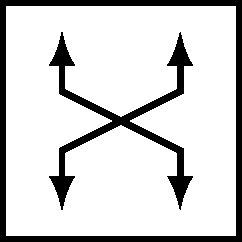
\includegraphics[width=0.9cm]{../common/fig-switch.pdf}
}
\providecommand{\router}{%
    
\includegraphics[width=0.9cm]{../common/fig-router.pdf}
}

\begin{frame}{basic flooding}
    \begin{itemize}
    \item idea: broadcast message to whole network
    \item where message comes from = way to send back
    \vspace{.5cm}
    \item used this idea in MAC learning
    \end{itemize}
\end{frame}

\begin{frame}{flooding one entry}
\begin{tikzpicture}
\tikzset{
    computer/.style={inner sep=0mm,outer sep=0mm,execute at begin node={\computer}},
    switch/.style={inner sep=0mm,outer sep=0mm,execute at begin node={\switch}},
    connect/.style={draw,very thick,Latex-Latex},
    connect big/.style={draw,ultra thick,Latex-Latex},
    port/.style={pos=0.95,fill=white,circle,draw,inner sep=0mm},
    port beginning/.style={pos=0.05,fill=white,circle,draw,inner sep=0mm},
    route table/.style={
        matrix of nodes,ampersand replacement=\&,
        column 1/.style={nodes={draw,thick,text width=2.5cm,font=\tiny\tt,text depth=0mm,minimum height=0.5cm,inner sep=1mm}},
        column 2/.style={nodes={draw,thick,text width=.5cm,font=\small\tt,text depth=0mm,minimum height=0.5cm,inner sep=1mm}},
        row 1/.style={nodes={draw=none,font=\small}},
    },
    mac label/.style={
        draw,fill=white,inner sep=1mm,font=\tiny\tt,
    },
}
\foreach \x/\d/\mc/\dir in {15/8cm/AA/north,45/3cm/BB/north,90/2cm/CC/north,135/3cm/DD/north,180/4cm/EE/north,300/4cm/FF/south} {
    \node[computer,label={[mac label,]\dir:00:11:22:33:44:\small\mc}] (c-\x) at (\x:\d) {};
}
\node[switch] (s1) at (4,-0.5) {};
\matrix[route table,anchor=north west,
    row 3/.style={nodes={visible on=<2->,alt=<2>{fill=red!10}}},
] (s1 table) at ([xshift=1cm,yshift=.5cm]s1.north east) {
dst MAC addr \& port \\
\ldots \& \ldots \\
00:11:22:33:44:\small AA \& 1 \\
};
\draw[dotted,thick] (s1.north east) -- (s1 table-2-1.north west);
\draw[dotted,thick] (s1.south east) -- (s1 table-2-1.south west);
\node[switch] (s2) at (-1,0.5) {};
\matrix[route table,
    row 3/.style={nodes={visible on=<3->}},
,anchor=north east] (s2 table) at ([xshift=3cm]s2.south west) {
dst MAC addr \& port \\
\ldots \& \ldots \\
00:11:22:33:44:\small AA \& 1 \\
};
\draw[dotted,thick] (s2.south east) -- (s2 table-2-2.north east);
\draw[dotted,thick] (s2.south west) -- (s2 table-2-1.north west);
\node[switch] (s3) at (-4,-3) {};
\matrix[route table,
    row 3/.style={nodes={visible on=<4->}},
,anchor=north west] (s3 table) at ([xshift=1cm,yshift=0.5cm]s3.north east) {
dst MAC addr \& port \\
\ldots \& \ldots \\
00:11:22:33:44:\small AA \& 2 \\
};
\draw[dotted,thick] (s3.south east) -- (s3 table-2-2.north east);
\draw[dotted,thick] (s3.south west) -- (s3 table-2-1.north west);
\draw[connect] (c-15) -- (s1) node[port] {1}
    node[midway,visible on=<2>,draw=red,fill=red!10] {from \ldots:AA};
\draw[connect] (c-45) -- (s1) node[port] {2};
\draw[connect] (c-300) -- (s1) node[port] {3};
\draw[connect] (c-90) -- (s2) node[port] {2};
\draw[connect] (c-135) -- (s2) node[port] {3};
\draw[connect] (c-180) -- (s2) node[port] {4};
\draw[connect big] (s1) -- (s2) node[port beginning] {4} node [port] {1}
    node[midway,visible on=<3>,draw=red,fill=red!10] {from \ldots:AA};
\draw[connect big] (s2) -- (s3) node[port beginning] {5} node [port] {2}
    node[midway,visible on=<4>,draw=red,fill=red!10] {from \ldots:AA};
\end{tikzpicture}
\end{frame}

\begin{frame}{`flooding'}
\begin{tikzpicture}
\tikzset{
    computer/.style={inner sep=0mm,outer sep=0mm,execute at begin node={\computer}},
    switch/.style={inner sep=0mm,outer sep=0mm,execute at begin node={\switch}},
    router/.style={inner sep=0mm,outer sep=0mm,execute at begin node={\router}},
    connect/.style={draw,very thick,Latex-Latex},
    connect big/.style={draw,ultra thick,Latex-Latex},
    port/.style={pos=0.95,fill=white,circle,draw,inner sep=0mm},
    port beginning/.style={pos=0.05,fill=white,circle,draw,inner sep=0mm},
    route table/.style={
        matrix of nodes,ampersand replacement=\&,
        column 1/.style={nodes={draw,thick,text width=2.2cm,font=\fontsize{7}{8}\selectfont\tt\strut,minimum height=0.4cm,inner sep=.2mm}},
        column 2/.style={nodes={draw,thick,text width=2.1cm,font=\fontsize{7}{8}\selectfont\tt\strut,minimum height=0.4cm,inner sep=.2mm}},
        column 3/.style={nodes={draw,thick,text width=.7cm,font=\fontsize{7}{8}\selectfont\tt\strut,minimum height=0.4cm,inner sep=.2mm}},
        row 1/.style={nodes={draw=none,font=\fontsize{9}{10}\selectfont}},
    },
    mac label/.style={
        draw,fill=white,inner sep=1mm,font=\tiny\tt,
    },
    s label/.style={
        font=\fontsize{8}{9}\tt\selectfont,align=center
    },
    net cloud/.style={cloud,draw,very thick,aspect=2},
    send out/.style={draw=violet,line width=1.5mm,dotted,-Latex},
    sent out info/.style={solid,draw=violet,line width=1mm,fill=white,align=left,font=\small\tt},
}
\node[router,label={[s label]north:(0) 2001:db8:1::1\\(1) 2001:db8:f::1},
    alt=<5>{fill=red!10},] (s1) at (3, 2) {};
\node[net cloud] (s1 cloud) at (1, 2.5) {};
\draw[connect] (s1) -- (s1 cloud) node[port beginning] {0};
\matrix[route table,anchor=north east] (s1 table) at ([xshift=-1cm]s1.north west) {
    addresses \& gateway \& port \\
    2001:db8:1::/40 \& --- \& 0 \\
    2001:db8:f::/40 \& --- \& 1 \\
};
\node[router,label={[s label]south:(0) 2001:db8:f::2\\(1) 2001:db8:2::1}] (s2) at (3, 0) {};
\draw[connect] (s1) -- (s2) node[port beginning] {1} node[port] {0};
\node[net cloud] (s2 cloud) at (6, 0) {};
\draw[connect] (s2) -- (s2 cloud) node[port beginning] {1};
\matrix[route table,anchor=north east,
    row 4/.style={nodes={visible on=<4->,alt=<4>{fill=red!10}}},
    row 5/.style={nodes={visible on=<5->,alt=<5>{fill=red!10}}},
] (s2 table) at ([xshift=-1cm]s2.north west) {
    addresses \& gateway \& port \\
    2001:db8:f::/40 \& --- \& 0 \\
    2001:db8:2::/40 \& --- \& 1 \\
    2001:db8:4::/40 \& 2001::db8:2::3 \& 1 \\
    2001:db8:1::/40 \& 2001::db8:f::1 \& 0 \\
};
\node[router,label={[s label]east:(0) 2001:db8:2::2\\(1) 2001:db8:3::1}] (s3) at (6, 1.5) {};
\draw[connect] (s2 cloud) -- (s3) node[port] {0};
\matrix[route table,anchor=south,
    row 4/.style={nodes={visible on=<4->,alt=<4>{fill=red!10}}},
    row 5/.style={nodes={visible on=<6->}},
    row 6/.style={nodes={visible on=<6->}},
    overlay,
    alt={<6>{row 5/.style={nodes={fill=red!10}}}},
    alt={<6>{row 6/.style={nodes={fill=red!10}}}},
] (s3 table) at ([xshift=1.5cm]s3.north) {
    addresses \& gateway \& port \\
    2001:db8:2::/40 \& --- \& 0 \\
    2001:db8:3::/40 \& --- \& 1 \\
    2001:db8:4::/40 \& 2001:db8:2::3\& 0 \\
    2001:db8:f::/40 \& 2001:db8:2::1\& 0 \\
    2001:db8:1::/40 \& 2001:db8:2::1\& 0 \\
};
\node[router,alt=<2-3>{fill=red!10},
      label={[s label]east:(0) 2001:db8:2::3\\(1) 2001:db8:4::1}] (s4) at (6, -1.5) {};
\draw[connect] (s2 cloud) -- (s4) node[port,alt=<2-3>{fill=red!10}] {0};
\matrix[
    route table,anchor=north,
    row 3/.style={nodes={visible on=<2->}},
    row 4/.style={nodes={visible on=<6->}},
    row 5/.style={nodes={visible on=<6->}},
    alt={<2-4>{row 3/.style={nodes={fill=red!10}}}},
    alt={<6>{row 4/.style={nodes={fill=red!10}}}},
    alt={<6>{row 5/.style={nodes={fill=red!10}}}},
] (s4 table) at (s4.south) {
    addresses \& gateway \& port \\
    2001:db8:2::/40 \& --- \& 0 \\
    2001:db8:4::/40 \& 2001:db8:2::3 \& 1 \\
    2001:db8:f::/40 \& 2001:db8:2::1 \& 0 \\
    2001:db8:1::/40 \& 2001:db8:2::1 \& 0 \\
};
    \begin{visibleenv}<2>
        \node[align=left,font=\small,fill=white,anchor=west,draw=red,ultra thick] at (s3.south west) {
            find out where \\
            we can forward packets \\
            not using port 0
        };
    \end{visibleenv}
    \begin{visibleenv}<3-4>
        \draw[send out] (s4.north) -- (s2 cloud.center) -- (s2);
        \draw[send out] (s4.north) -- (s2 cloud.center) -- (s3);
        \node[sent out info,anchor=north west] at ([xshift=.5cm]s3.south) {
            via 2001:db8:2::3 \\
            2001:db8:3::/40
        };
    \end{visibleenv}
    \begin{visibleenv}<5>
        \draw[send out] (s1.south) -- (s2.north)
            node[midway, left=1cm, sent out info] {
                via 2001:db8:f::1 \\
                2001:db8:1::/40
            };
    \end{visibleenv}
    \begin{visibleenv}<6>
        \draw[send out] (s2.east) -- (s2 cloud.center) -- (s3.south);
        \draw[send out] (s2.east) -- (s2 cloud.center) -- (s4.north);
        \node[anchor=west,sent out info] at (s2 cloud.east)
            {
                via 2001:db8:2::1 \\
                2001::db8:f::/40 \\
                2001::db8:1::/40 
            };
    \end{visibleenv}
\end{tikzpicture}
\end{frame}

\begin{frame}{eventual convergence}
    \begin{itemize}
    \item `flooding' algorithm:
    \item periodically send on each network:
        \begin{itemize}
        \item list of routes you have that don't double-back to same network
        \end{itemize}
    \item when receiving routes sent on network:
        \begin{itemize}
        \item add routing table entry for each route
        \end{itemize}
    \vspace{.5cm}
    \item<2-> not handled: \myemph{multiple paths}?
    \end{itemize}
\end{frame}

\begin{frame}{only one path?}
    \begin{itemize}
    \item only one path on network means:
    \vspace{.5cm}
    \item if a link fails, bad news
    \item network forms a tree
    \end{itemize}
\end{frame}

\begin{frame}{routing like this?}
    \begin{itemize}
    \item for IP routing, generally want to have multiple paths
    \item \ldots but this is basically how MAC learning works
    \vspace{.5cm}
    \item but it requires a network that is a tree
    \item what if we don't start with one?
    \end{itemize}
\end{frame}


\section{spanning trees}
\usetikzlibrary{arrows.meta,calc,matrix,shapes}
\providecommand{\computer}{%
    
\includegraphics[width=1cm]{../common/Noun_project_216.pdf}
}
\providecommand{\switch}{%
    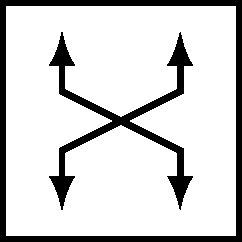
\includegraphics[width=0.9cm]{../common/fig-switch.pdf}
}
\providecommand{\router}{%
    
\includegraphics[width=0.9cm]{../common/fig-router.pdf}
}

\begin{frame}{spanning tree}
    \begin{itemize}
    \item given a general network, only activate subset of links
    \item \ldots such that network is tree
        \begin{itemize}
        \item that is only one path between each node
        \end{itemize}
    \vspace{.5cm}
    \item allows us to do flooding strategy
    \item makes simple MAC learning/broadcast just work
    \end{itemize}
\end{frame}

\begin{frame}{centralized spanning tree?}
    \begin{itemize}
    \item one algorithm you might learn in DSA2:
    \vspace{.5cm}
    \item mark one node called \textit{the root} as `in the tree'
    \item repeatedly: 
        \begin{itemize}
        \item add the `\myemph<2>{first}' link that goes to a node not in the tree
        \item mark newly connected node as `in the tree'
        \end{itemize}
    \vspace{.5cm}
    \item result = spanning tree
    \end{itemize}
\end{frame}

\begin{frame}{a careful ordering}
    \begin{itemize}
    \item algorithm works with any idea of which link/node is first
    \vspace{.5cm}
    \item we'll choose a particular ordering (for reasons you'll see later)
    \vspace{.5cm}
    \item first node one with earliest `name'
    \item links closer to the root before further links
    \item links from nodes with earlier names before later ones
    \end{itemize}
\end{frame}

\begin{frame}[fragile]{spanning tree example}
\begin{tikzpicture}
\tikzset{
    computer/.style={inner sep=0mm,outer sep=0mm,execute at begin node={\computer}},
    switch/.style={inner sep=0mm,outer sep=0mm,execute at begin node={\switch}},
    port/.style={pos=0.95,fill=white,circle,draw,inner sep=0mm},
    port beginning/.style={pos=0.05,fill=white,circle,draw,inner sep=0mm},
    route table/.style={
        matrix of nodes,ampersand replacement=\&,
        column 1/.style={nodes={draw,thick,text width=2.5cm,font=\tiny\tt,text depth=0mm,minimum height=0.5cm,inner sep=1mm}},
        column 2/.style={nodes={draw,thick,text width=.5cm,font=\small\tt,text depth=0mm,minimum height=0.5cm,inner sep=1mm}},
        row 1/.style={nodes={draw=none,font=\small}},
    },
    mac label/.style={
        draw,fill=white,inner sep=1mm,font=\tiny\tt,
    },
    tn/.style={draw,dotted,circle,very thick},
    real at/.style={alt=<#1->{solid},alt=<#1>{fill=red!10}},
    connect maybe/.style={draw,very thick,dotted,Latex-Latex},
    actual at/.style={alt=<#1->{draw=red,solid},alt=<#1>{draw,solid}},
    consider at/.style={alt=<#1>{draw=red}},
}
\node[tn,real at=1] (A) at (0, 0) {A};
\node[tn,real at=3] (B) at (5, -1) {B};
\node[tn,real at=4] (G) at (-5, -1) {G};
\node[tn,real at=6] (D) at (7, -3) {D};
\node[tn,real at=7] (E) at (1, -5) {E};
\node[tn,real at=8] (F) at (-7, -4) {F};
\draw[connect maybe,consider at=2,actual at=3] (A) -- (B)
    node[midway,sloped,above,visible on=<2>] {first priority};
\draw[connect maybe,consider at=2,actual at=4] (A) -- (G)
    node[midway,sloped,above,visible on=<2>] {second priority};
\draw[connect maybe,consider at=5] (B) -- (G)
    node[midway,sloped,below,visible on=<5>] {no new nodes};
\draw[connect maybe,actual at=6,consider at=5] (B) -- (D)
    node[midway,below left,visible on=<5>] {first priority};
\draw[connect maybe,actual at=8,consider at=5] (G) -- (F)
    node[midway,below right,visible on=<5>] {second priority};
\draw[connect maybe,consider at=6,actual at=7] (G) -- (E);
\draw[connect maybe,consider at=6] (D) -- (E);
\draw[connect maybe] (E) -- (F);
\end{tikzpicture}
\end{frame}

\begin{frame}{detecting `mistakes'}
    \begin{itemize}
    \item this method: consistent results every time
    \vspace{.5cm}
    \item but assumes we start from scratch
    \item we're going to want a way of doing this dynamically
    \vspace{.5cm}
    \item let's say we find a wrong configuration ---
    \item can we fix it?
    \end{itemize}
\end{frame}

\begin{frame}[fragile]{fixing wrong links}
\begin{tikzpicture}
\tikzset{
    computer/.style={inner sep=0mm,outer sep=0mm,execute at begin node={\computer}},
    switch/.style={inner sep=0mm,outer sep=0mm,execute at begin node={\switch}},
    port/.style={pos=0.95,fill=white,circle,draw,inner sep=0mm},
    port beginning/.style={pos=0.05,fill=white,circle,draw,inner sep=0mm},
    route table/.style={
        matrix of nodes,ampersand replacement=\&,
        column 1/.style={nodes={draw,thick,text width=2.5cm,font=\tiny\tt,text depth=0mm,minimum height=0.5cm,inner sep=1mm}},
        column 2/.style={nodes={draw,thick,text width=.5cm,font=\small\tt,text depth=0mm,minimum height=0.5cm,inner sep=1mm}},
        row 1/.style={nodes={draw=none,font=\small}},
    },
    mac label/.style={
        draw,fill=white,inner sep=1mm,font=\tiny\tt,
    },
    tn/.style={draw,dotted,circle,very thick},
    n real/.style={solid},
    n real at/.style={alt=<#1->{solid},alt=<#1>{fill=red!10}},
    n real until/.style={alt=<1-#1>{solid}},
    connect maybe/.style={draw,very thick,dotted,Latex-Latex},
    e real at/.style={alt=<#1>{draw=red,solid},alt=<#1->{draw,solid}},
    e real until/.style={alt=<1-#1>{solid},alt=<#1>{draw=red,solid}},
    e real/.style={solid},
    e hide up to/.style={alt=<1-#1>{invisible}},
    consider at/.style={alt=<#1>{draw=red,dotted}},
    explain box/.style={at={(0, -4)},align=center,draw=red,ultra thick,fill=white},
    explain box up/.style={at={(2, -1)},align=center,draw=red,ultra thick,fill=white},
}
\node[tn,n real] (A) at (0, 0) {A};
\node[tn,n real] (B) at (5, -1) {B};
\node[tn,n real] (G) at (-5, -1) {G};
\node[tn,n real] (D) at (7, -3) {D};
\node[tn,n real] (E) at (1, -5) {E};
\node[tn,n real] (F) at (-7, -4) {F};
\draw[connect maybe,e real] (A) -- (B);
\draw[connect maybe,e hide up to=1,e real at=2,consider at=2,alt=<3->{draw=black}] (A) -- (G);
\draw[connect maybe,e real until=2] (B) -- (G);
\draw[connect maybe,e real] (B) -- (D);
\draw[connect maybe,e real] (G) -- (F);
\draw[connect maybe,e hide up to=4,e real at=5] (G) -- (E);
\draw[connect maybe,e hide up to=2,alt=<3-4>{solid},alt=<3>{red},alt=<5>{red}] (D) -- (E);
\draw[connect maybe,e real until=3] (E) -- (F);
\begin{visibleenv}<2>
\node[explain box] {
    A--G beats B--G: closer to root
};
\end{visibleenv}
\begin{visibleenv}<3>
\node[explain box up] {
    D--F and F--E: \\
    same distance from root, but \\
    D before F, so D--E beats F--E
};
\end{visibleenv}
\begin{visibleenv}<5>
\node[explain box up] {
    G--E and D--E: \\
    G--E closer to root \\
    so G--E beats D--E
};
\end{visibleenv}
\end{tikzpicture}
\end{frame}

\begin{frame}{spanning tree protocol}
    \begin{itemize}
    \item each node tracks:
        \begin{itemize}
        \item what it believes is root of tree
        \item its link toward root of tree
        \item its distance to root of tree
        \item which other nodes think it's closer to root of tree
        \end{itemize}
    \item periodically sends information to neighbors
    \item when receiving information, update:
        \begin{itemize}
        \item root to lower ID number (if possible)
        \item link to lower-distance link  (if possible)
        \item link to lower-ID, same-distance link (if possible)
        \item which other nodes think it is closer
        \end{itemize}
    \end{itemize}
\end{frame}

\begin{frame}[fragile]{some example updates}
\begin{tikzpicture}
\tikzset{
    computer/.style={inner sep=0mm,outer sep=0mm,execute at begin node={\computer}},
    switch/.style={inner sep=0mm,outer sep=0mm,execute at begin node={\switch}},
    port/.style={pos=0.95,fill=white,circle,draw,inner sep=0mm},
    port beginning/.style={pos=0.05,fill=white,circle,draw,inner sep=0mm},
    route table/.style={
        matrix of nodes,ampersand replacement=\&,
        column 1/.style={nodes={draw,thick,text width=2.5cm,font=\tiny\tt,text depth=0mm,minimum height=0.5cm,inner sep=1mm}},
        column 2/.style={nodes={draw,thick,text width=.5cm,font=\small\tt,text depth=0mm,minimum height=0.5cm,inner sep=1mm}},
        row 1/.style={nodes={draw=none,font=\small}},
    },
    mac label/.style={
        draw,fill=white,inner sep=1mm,font=\tiny\tt,
    },
    n real/.style={solid},
    n real at/.style={alt=<#1->{solid},alt=<#1>{fill=red!10}},
    n real until/.style={alt=<1-#1>{solid}},
    tn/.style={draw,dotted,circle,very thick},
    real at/.style={alt=<#1->{solid},alt=<#1>{fill=red!10}},
    connect maybe/.style={draw,very thick,dotted,Latex-Latex},
    actual at/.style={alt=<#1->{draw=red,solid},alt=<#1>{draw,solid}},
    consider at/.style={alt=<#1>{draw=red}},
    msg link/.style={draw,violet,line width=1.2mm,-Latex},
    msg data/.style={draw=violet,line width=1mm,fill=white,align=left},
}
\node[tn,n real] (A) at (0, 0) {A};
\node[tn,n real] (B) at (5, -1) {B};
\node[tn,n real] (G) at (-5, -1) {G};
\node[tn,n real] (D) at (7, -3) {D};
\node[tn,n real] (E) at (1, -5) {E};
\node[tn,n real] (F) at (-7, -4) {F};
\draw[connect maybe] (A) -- (B);
\draw[connect maybe] (A) -- (G);
\draw[connect maybe] (B) -- (G);
\draw[connect maybe] (B) -- (D);
\draw[connect maybe] (G) -- (F);
\draw[connect maybe] (G) -- (E);
\draw[connect maybe] (D) -- (E);
\draw[connect maybe] (E) -- (F);
\tikzset{
    every node/.style={font=\small},
}
\begin{visibleenv}<2>
    \draw[msg link] (E) -- (G);
    \draw[msg link] (E) -- (F);
    \draw[msg link] (E) -- (D);
    \node[draw,very thick,anchor=south west] at (G.north east) {
        r=G,d=0,no link
    };
    \node[draw,very thick,alt=<2>{msg data},anchor=north] at (E.south) {
        r=E,d=0,no link
    };
    \node[draw,very thick,anchor=north west] at (F.south east) {
        r=F,d=0,no link
    };
    \node[draw,very thick,anchor=north west] at (D.south west) {
        r=D,d=0,no link
    };
\end{visibleenv}
\begin{visibleenv}<3>
    \draw[msg link] (E) -- (G);
    \draw[msg link] (E) -- (F);
    \draw[msg link] (E) -- (D);
    \node[draw,very thick,draw=red,anchor=south west] at (G.north east) {
        r=E,d=1,G--E
    };
    \node[draw,very thick,anchor=north] at (E.south) {
        r=E,d=0,no link
    };
    \node[draw,very thick,draw=red,anchor=north west] at (F.south east) {
        r=E,d=0,F--E
    };
    \node[align=left,draw,very thick,draw=red,anchor=north east] at (D.south west) {
        r=D,d=0,no link \\
        (D < G, so no update)
    };
\end{visibleenv}
\begin{visibleenv}<4>
    \draw[msg link] (D) -- (B);
    \draw[msg link] (D) -- (E);
    \node[draw,very thick,anchor=south west] at (G.north east) {
        r=E,d=1,G--E
    };
    \node[draw,very thick,anchor=north] at (E.south) {
        r=E,d=0,no link
    };
    \node[draw,very thick,anchor=north west] at (F.south east) {
        r=E,d=0,F--E
    };
    \node[draw,very thick,alt=<4>{msg data},anchor=north east] at (D.south west) {
        r=D,d=0,no link
    };
    \node[draw,very thick,anchor=south] at (B.north) {
        r=B,d=0,no link
    };
\end{visibleenv}
\begin{visibleenv}<5>
    \draw[msg link] (D) -- (B);
    \draw[msg link] (D) -- (E);
    \node[draw,very thick,anchor=south west] at (G.north east) {
        r=E,d=1,G--E
    };
    \node[draw,very thick,draw=red,anchor=north] at (E.south) {
        r=D,d=1,E--D
    };
    \node[draw,very thick,anchor=north west] at (F.south east) {
        r=E,d=0,F--E
    };
    \node[draw,very thick,anchor=north east] at (D.south west) {
        r=D,d=0,no link
    };
    \node[align=left,draw,very thick,draw=red,anchor=south] at (B.north) {
        r=B,d=0,no link \\
        (B < D, no update)
    };
\end{visibleenv}
\end{tikzpicture}
\end{frame}

\begin{frame}{spanning trees in practice (1)}
    \begin{itemize}
    \item commonly used on Ethernet for switches
    \item links not in spanning tree are `blocked'
        \begin{itemize}
        \item not used for normal traffic
        \item assumption: would cause loop $\rightarrow$ infinite packets
        \end{itemize}
    \item delay before activating port
        \begin{itemize}
        \item avoid temporary routing loops while figuring out tree
        \end{itemize}
    \item periodically send updates to all neighbors
        \begin{itemize}
        \item order of seconds
        \end{itemize}
    \end{itemize}
\end{frame}

\begin{frame}{spanning tree in practice (2)}
    \begin{itemize}
    \item real protocol supports variable `cost' for links
        \begin{itemize}
        \item so `distance to root' might be lower for faster links
        \end{itemize}
    \item modern variant (Rapid Spanning Tree Protocol) selects ``backup'' port to root 
        \begin{itemize}
        \item goal: faster switchover on failure
        \end{itemize}
    \end{itemize}
\end{frame}


\section{preview: better routing}
\begin{frame}[fragile]{exercise: best routes?}
\begin{tikzpicture}
\tikzset{
    computer/.style={inner sep=0mm,outer sep=0mm,execute at begin node={\computer}},
    switch/.style={inner sep=0mm,outer sep=0mm,execute at begin node={\switch}},
    port/.style={pos=0.95,fill=white,circle,draw,inner sep=0mm},
    port beginning/.style={pos=0.05,fill=white,circle,draw,inner sep=0mm},
    route table/.style={
        matrix of nodes,ampersand replacement=\&,
        column 1/.style={nodes={draw,thick,text width=2.5cm,font=\tiny\tt,text depth=0mm,minimum height=0.5cm,inner sep=1mm}},
        column 2/.style={nodes={draw,thick,text width=.5cm,font=\small\tt,text depth=0mm,minimum height=0.5cm,inner sep=1mm}},
        row 1/.style={nodes={draw=none,font=\small}},
    },
    mac label/.style={
        draw,fill=white,inner sep=1mm,font=\tiny\tt,
    },
    n real/.style={solid},
    n real at/.style={alt=<#1->{solid},alt=<#1>{fill=red!10}},
    n real until/.style={alt=<1-#1>{solid}},
    tn/.style={draw,dotted,circle,very thick},
    real at/.style={alt=<#1->{solid},alt=<#1>{fill=red!10}},
    connect maybe/.style={draw,very thick,dotted,Latex-Latex},
    actual at/.style={alt=<#1->{draw=red,solid},alt=<#1>{draw,solid}},
    consider at/.style={alt=<#1>{draw=red}},
    msg link/.style={draw,violet,line width=1.2mm,-Latex},
    msg data/.style={draw=violet,line width=1mm,fill=white,align=left},
}
\node[tn,n real] (A) at (0, 0) {A};
\node[tn,n real] (B) at (5, -1) {B};
\node[tn,n real] (G) at (-5, -1) {G};
\node[tn,n real] (D) at (7, -3) {D};
\node[tn,n real] (E) at (1, -5) {E};
\node[tn,n real] (F) at (-7, -4) {F};
\draw[connect maybe] (A) -- (B) node[midway,sloped,above] {1Mbit, 10ms};
\draw[connect maybe] (A) -- (G) node[midway,sloped,above] {10Mbit, 20ms};
\draw[connect maybe] (B) -- (G) node[midway,sloped,above] {11Mbit, 20ms};
\draw[connect maybe] (B) -- (D) node[midway,sloped,above] {5Mbit, 100ms};
\draw[connect maybe] (G) -- (F) node[midway,sloped,above] {6Mbit, 5ms};
\draw[connect maybe] (G) -- (E) node[midway,sloped,above] {8Mbit, 10ms};
\draw[connect maybe] (D) -- (E) node[midway,sloped,above] {2Mbit, 20ms};
\draw[connect maybe] (E) -- (F) node[midway,sloped,above] {100Mbit, 10ms};
\end{tikzpicture}
\begin{itemize}
\item A to B? B to E? F to G?
\end{itemize}
\end{frame}


\section{aside: metrics}
\begin{frame}{routing metrics}
    \begin{itemize}
    \item want some way of saying how `good' link is
    \item typically ``cost''/``distance'' value (so lower is better)
    \item in practice, most commonly \[\frac{\text{constant}}{\text{bandwidth}}\]
    \vspace{.5cm}
    \item could also try to:
        \begin{itemize}
        \item take financial costs into account
        \item take lantency into account
        \item take reliability into account
        \item spread flows out among more links
        \end{itemize}
    \end{itemize}
\end{frame}


\section{Bellman-Ford}
\usetikzlibrary{arrows.meta,matrix}
\begin{frame}{all-pairs Bellman-Ford}
    \begin{itemize}
    \item one algorithm to find all shortest paths in graph (network)
    \vspace{.5cm}
    \item $d(A,B) = \text{best distance from A to B}$
    \item $p(A,B) = \text{next node on path from A to B}$
    \item initially $d(X,X) = \infty$ for all nodes $X$
    \item repeatedly* do the following:
    \vspace{.5cm}
    \item for each link from A to B, distance $c$:
        \begin{itemize}
        \item for each node X:
        \item if $c + d(B, X) < d(A, X)$, \\
        \item then $d(A,X) \leftarrow c+d(B,X)$, $p(A,X) = B$
        \end{itemize}
    \end{itemize}
\end{frame}

\providecommand{\noroute}{$\infty$/---}
\providecommand{\mymark}[2]{\alt<#1->{\myemph<#1>{#2}}{}}
\begin{frame}[fragile]{running Bellman-Ford}
\begin{tikzpicture}
\tikzset{
    computer/.style={inner sep=0mm,outer sep=0mm,execute at begin node={\computer}},
    switch/.style={inner sep=0mm,outer sep=0mm,execute at begin node={\switch}},
    port/.style={pos=0.95,fill=white,circle,draw,inner sep=0mm},
    port beginning/.style={pos=0.05,fill=white,circle,draw,inner sep=0mm},
    route table/.style={
        matrix of nodes,ampersand replacement=\&,
        column 1/.style={nodes={draw,thick,text width=2.5cm,font=\tiny\tt,text depth=0mm,minimum height=0.5cm,inner sep=1mm}},
        column 2/.style={nodes={draw,thick,text width=.5cm,font=\small\tt,text depth=0mm,minimum height=0.5cm,inner sep=1mm}},
        row 1/.style={nodes={draw=none,font=\small}},
    },
    mac label/.style={
        draw,fill=white,inner sep=1mm,font=\tiny\tt,
    },
    n real/.style={solid},
    n real at/.style={alt=<#1->{solid},alt=<#1>{fill=red!10}},
    n real until/.style={alt=<1-#1>{solid}},
    tn/.style={draw,dotted,circle,very thick},
    real at/.style={alt=<#1->{solid},alt=<#1>{fill=red!10}},
    connect/.style={draw,very thick,-Latex},
    connect big/.style={draw,ultra thick,-Latex},
    actual at/.style={alt=<#1->{draw=red,solid},alt=<#1>{draw,solid}},
    consider at/.style={alt=<#1>{draw=red}},
    msg link/.style={draw,violet,line width=1.2mm,-Latex},
    msg data/.style={draw=violet,line width=1mm,fill=white,align=left},
}
\begin{scope}[x=0.8cm]
\node[tn,n real] (A) at (0, 0) {A};
\node[tn,n real] (B) at (5, -2) {B};
\node[tn,n real] (C) at (-5, -2) {C};
\node[tn,n real] (D) at (0, -4) {D};
\draw[connect big,alt=<2>{red}] ([yshift=1mm]A.east) -- ([xshift=1mm]B.north) node[midway,above] {2};
\draw[connect,alt=<3>{red},alt=<8>{red}] ([xshift=-1mm]B.north) -- ([yshift=-1mm]A.east) node[midway,below] {4};
\draw[connect big,alt=<7>{red}] ([yshift=1mm]A.west) -- ([xshift=-1mm]C.north) node[midway,above] {1};
\draw[connect big] ([xshift=1mm]C.north) -- ([yshift=-1mm]A.west) node[midway,below] {2};
\draw[connect big,alt=<5>{red}] ([yshift=1mm]C.east) -- ([yshift=1mm]B.west) node[midway,above] {2};
\draw[connect big,alt=<4>{red}] ([yshift=-1mm]B.west) -- ([yshift=-1mm]C.east) node[midway,below] {2};
\draw[connect,alt=<6>{red}] ([xshift=1mm]C.south) -- ([yshift=1mm]D.west) node[midway,above] {4};
\draw[connect] ([yshift=-1mm]D.west) -- ([xshift=-1mm]C.south) node[midway,below] {5};
\draw[connect big] ([xshift=-1mm]B.south) -- ([yshift=1mm]D.east) node[midway,above] {1};
\draw[connect big] ([yshift=-1mm]D.east) -- ([xshift=1mm]B.south) node[midway,below] {2};
\begin{visibleenv}<1-9>
\matrix[anchor=north west,tight matrix,
    nodes={font=\fontsize{10}{11}\selectfont,text width=1cm,minimum height=0.5cm}
] at (6, 0) {
    ~ \& A \& B \& C \& D \\
    A \& |[alt=<3>{fill=red!10}]| 0/A \& \only<1>{\noroute}\mymark{2}{2/B} \& \only<1-6>{\noroute}\mymark{7}{1/C} \& \only<1-6>{\noroute}\mymark{7}{5/D} \\
    B \& |[alt=<5>{fill=red!10}]| \only<1-2>{\noroute}\mymark{3}{4/A} \& |[alt=<2>{fill=red!10},alt=<5>{fill=red!10}]| 0/B\& \only<1-3>{\noroute}\mymark{4}{2/C} \& \only<1-7>{\noroute}{\mymark{8}{9/A}} \\
    C \& \only<1-4>{\noroute}\only<5->{\mymark{5}{6/B}} \& \only<1-4>{\noroute}\mymark{5}{2/B} \& 0/C \& 
            \only<1-5>{\noroute}{\mymark{6}{4/D}} \\
    D \& \noroute \& \noroute \& \noroute \& 0/D \\
};
\end{visibleenv}
\begin{visibleenv}<10>
\matrix[anchor=north west,tight matrix,
    nodes={font=\fontsize{10}{11}\selectfont,text width=1cm,minimum height=0.5cm}
] at (6, 0) {
    ~ \& A \& B \& C \& D \\
    A \& 0/A \& 2/B \& 4/C \& 3/B \\
    B \& 4/A \& 0/B \& 2/C \& 1/D \\
    C \& 2/A \& 2/B \& 0/C \& 4/D \\
    D \& 6/B \& 2/B \& 4/B \& 0/D \\
};
\end{visibleenv}
\end{scope}
\end{tikzpicture}
\end{frame}


\section{distance vector routing}
\subsection{distributing Bellman-Ford}
\usetikzlibrary{arrows.meta,matrix}

\providecommand{\noroute}{$\infty$/---}
\providecommand{\mymark}[2]{\alt<#1->{\myemph<#1>{#2}}{}}
\begin{frame}[fragile]{distributing Bellman-Ford}
\begin{tikzpicture}
\tikzset{
    computer/.style={inner sep=0mm,outer sep=0mm,execute at begin node={\computer}},
    switch/.style={inner sep=0mm,outer sep=0mm,execute at begin node={\switch}},
    port/.style={pos=0.95,fill=white,circle,draw,inner sep=0mm},
    port beginning/.style={pos=0.05,fill=white,circle,draw,inner sep=0mm},
    route table/.style={
        matrix of nodes,ampersand replacement=\&,
        column 1/.style={nodes={draw,thick,text width=2.5cm,font=\tiny\tt,text depth=0mm,minimum height=0.5cm,inner sep=1mm}},
        column 2/.style={nodes={draw,thick,text width=.5cm,font=\small\tt,text depth=0mm,minimum height=0.5cm,inner sep=1mm}},
        row 1/.style={nodes={draw=none,font=\small}},
    },
    mac label/.style={
        draw,fill=white,inner sep=1mm,font=\tiny\tt,
    },
    n real/.style={solid},
    n real at/.style={alt=<#1->{solid},alt=<#1>{fill=red!10}},
    n real until/.style={alt=<1-#1>{solid}},
    tn/.style={draw,dotted,circle,very thick},
    real at/.style={alt=<#1->{solid},alt=<#1>{fill=red!10}},
    connect/.style={draw,very thick,-Latex},
    connect big/.style={draw,ultra thick,-Latex},
    actual at/.style={alt=<#1->{draw=red,solid},alt=<#1>{draw,solid}},
    consider at/.style={alt=<#1>{draw=red}},
    msg link/.style={draw,violet,line width=1.2mm,-Latex},
    msg data/.style={draw=violet,line width=1mm,fill=white,align=left},
}
\begin{scope}[x=0.8cm]
\node[tn,n real] (A) at (0, 0) {A};
\node[tn,n real] (B) at (5, -2) {B};
\node[tn,n real] (C) at (-5, -2) {C};
\node[tn,n real] (D) at (0, -4) {D};
\draw[connect big] ([yshift=1mm]A.east) -- ([xshift=1mm]B.north) node[midway,above] {2};
\draw[connect] ([xshift=-1mm]B.north) -- ([yshift=-1mm]A.east) node[midway,below] {4};
\draw[connect big] ([yshift=1mm]A.west) -- ([xshift=-1mm]C.north) node[midway,above] {1};
\draw[connect big] ([xshift=1mm]C.north) -- ([yshift=-1mm]A.west) node[midway,below] {2};
\draw[connect big] ([yshift=1mm]C.east) -- ([yshift=1mm]B.west) node[midway,above] {2};
\draw[connect big] ([yshift=-1mm]B.west) -- ([yshift=-1mm]C.east) node[midway,below] {2};
\draw[connect] ([xshift=1mm]C.south) -- ([yshift=1mm]D.west) node[midway,above] {4};
\draw[connect] ([yshift=-1mm]D.west) -- ([xshift=-1mm]C.south) node[midway,below] {5};
\draw[connect big] ([xshift=-1mm]B.south) -- ([yshift=1mm]D.east) node[midway,above] {1};
\draw[connect big] ([yshift=-1mm]D.east) -- ([xshift=1mm]B.south) node[midway,below] {2};
\matrix[anchor=north west,tight matrix,
    nodes={font=\fontsize{10}{11}\selectfont,text width=1cm,minimum height=0.5cm},
    alt=<2>{
        row 2/.style={nodes={fill=violet!10}},
    },
    alt=<2>{
        row 3/.style={nodes={fill=green!10}},
    },
    alt=<2>{
        row 4/.style={nodes={fill=blue!10}},
    },
    alt=<2>{
        row 5/.style={nodes={fill=yellow!10}},
    },
    overlay,
] at (4, 2) {
    ~ \& A \& B \& C \& D \\
    A \& 0/A \& 2/B \& 1/C \& 5/D \\
    B \& 4/A \& 0/B\& 2/C \& 6/C \\
    C \& 1/A \& 2/B \& 0/C \& 4/D \\
    D \& \noroute \& \noroute \& \noroute \& 0/D \\
};
\begin{visibleenv}<2->
\tikzset{
    one dv/.style={
        tight matrix,
        nodes={alt=<2>{draw=red},fill=white,font=\fontsize{10}{11}\selectfont,text width=1cm,minimum height=0.5cm}
    }
}
\matrix[anchor=south,one dv,
    row 2/.style={nodes={fill=violet!10}},
] (A dv) at (A.north) {
    A \& B \& C \& D \\
    0/A \& 2/B \& 1/C \& 5/D \\
};
\matrix[anchor=north,one dv,
    row 2/.style={nodes={fill=yellow!10}},
] (D dv) at ([yshift=0cm]D.south) {
    A \& B \& C \& D \\
    \only<1-3>{\noroute}\mymark{4}{6/C} \& \only<1-6>{\noroute}\mymark{6}{7/B} \& \only<1-3>{\noroute}\mymark{4}{5/C} \& 0/D \\
};
\matrix[anchor=south west,one dv,
    row 2/.style={nodes={fill=blue!10}},
] (C dv) at ([xshift=-3cm]C.north east) {
    A \& B \& C \& D \\
    1/A \& 2/B \& 0/C \& 4/D \\
};
\matrix[anchor=north east,one dv,
    row 2/.style={nodes={fill=green!10}},
] (B dv) at ([yshift=.25cm,xshift=4cm]B.south west) {
    A \& B \& C \& D \\
     4/A \& 0/B\& 2/C \& 6/C \\
};
\end{visibleenv}
\begin{visibleenv}<1>
\node[fill=white,anchor=north,draw=red,ultra thick,align=center] at (1, 1) {
    store table row = ``distance vector'' on each node
};
\end{visibleenv}
\begin{visibleenv}<3-4>
\draw[msg link] (C) -- (D)
    node[midway,above,msg data] {I'm C, costs: A=1,B=2,C=0,D=5};
\end{visibleenv}
\begin{visibleenv}<3>
\node[fill=white,anchor=north,draw=red,ultra thick,align=center] at (1, 1) {
    nodes share their `distance vector' periodically\ldots
};
\end{visibleenv}
\begin{visibleenv}<4>
\node[fill=white,anchor=north,draw=red,ultra thick,align=center] at (1, 1) {
    when receiving distance vector \\
    see if new node (C) has better routes
};
\end{visibleenv}
\begin{visibleenv}<5>
\draw[msg link] (B) -- (D)
    node[midway,above,msg data] {I'm B, costs: A=4,B=0,C=2,D=5};
\node[fill=white,anchor=north,draw=red,ultra thick,align=center] at (1, 1) {
    exercise: what should change from update?
};
\end{visibleenv}
\end{scope}
\end{tikzpicture}
\end{frame}



\subsection{aside: networks and routers}
\usetikzlibrary{fit,matrix}
\usetikzlibrary{arrows.meta,calc,shapes}
\providecommand{\computer}{%
    
\includegraphics[width=0.7cm]{../common/Noun_project_216.pdf}
}
\providecommand{\computerAlt}{%
    
\includegraphics[width=0.8cm]{../common/Noun_project_alt_cpu.pdf}
}
\providecommand{\switch}{%
    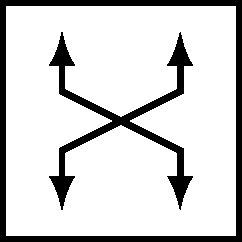
\includegraphics[width=0.8cm]{../common/fig-switch.pdf}
}
\providecommand{\router}{%
    
\includegraphics[width=0.8cm]{../common/fig-router.pdf}
}
\begin{frame}{networks v routers (DV)}
    \begin{itemize}
    \item imprecision on graphs --- acting as if we want distance to routers
    \item but really want distance to networks
    \vspace{.5cm}
    \item distance vectors will track distance to \textit{networks}
    \item but next hops will be routers
    \end{itemize}
\end{frame}

\begin{frame}[fragile]{networks v routers (DV)}
\tikzset{
    mynode/.style={draw,circle,very thick,font=\small},
    myedge/.style={draw,ultra thick},
    computer/.style={inner sep=0mm,outer sep=0mm,execute at begin node={\computer}},
    switch/.style={inner sep=0mm,outer sep=0mm,execute at begin node={\switch}},
    router/.style={inner sep=0mm,outer sep=0mm,execute at begin node={\router}},
    port/.style={pos=0.95,fill=white,circle,draw,inner sep=0mm},
    port beginning/.style={pos=0.05,fill=white,circle,draw,inner sep=0mm},
    connect/.style={draw,thick,Latex-Latex},
    msg link/.style={draw,violet,line width=1.2mm,-Latex},
    msg data/.style={draw=violet,line width=0.8mm,fill=white,align=left,font=\fontsize{9}{10}\selectfont,align=left},
}
\begin{tikzpicture}
\foreach \x/\offX/\offY in {1/0/0,2/3/0} {
    \begin{scope}[xshift=\offX cm,yshift=\offY cm]
    \node[computer] (c\x-a) at (0, 0) {};
    \node[computer] (c\x-b) at (1, 0) {};
    \node[switch] (s\x) at (0.5, -1) {};
    \draw[connect] (c\x-a) -- (s\x);
    \draw[connect] (c\x-b) -- (s\x);
    \end{scope}
}
\foreach \x/\offX/\offY in {3/0/-6} {
    \begin{scope}[xshift=\offX cm,yshift=\offY cm]
    \node[computer] (c\x-a) at (0, 0) {};
    \node[computer] (c\x-b) at (1, -.5) {};
    \node[computer] (c\x-c) at (2, -.5) {};
    \node[switch] (s\x) at (0.5, 2) {};
    \node[switch] (s\x-b) at (1.5, 1) {};
    \draw[connect] (c\x-a) -- (s\x);
    \draw[connect] (c\x-b) -- (s\x-b);
    \draw[connect] (c\x-c) -- (s\x-b);
    \draw[connect] (s\x) -- (s\x-b);
    \end{scope}
}
\node[switch] (s4) at (4, -5) {};
\node[router,label={south:R1}] (r1) at (-1, -3) {};
\node[router,label={south:R2}] (r2) at (2, -2) {};
\node[router,label={south:R3}] (r3) at (2, -3.4) {};
\node[router,label={south:R4}] (r4) at (5, -3.25) {};
\foreach \x/\y in {r1/s1,r2/s1,r2/s2,r3/s3,r2/s4,r1/s3,r3/s4,s3/r3,s2/r4,r4/s4} {
    \draw[connect] (\x) -- (\y);
}
\begin{visibleenv}<2->
\draw[dotted, very thick,fill=green,fill opacity=0.1,text opacity=1.] ([xshift=-.2cm]c1-a.north west) -- ([xshift=.2cm]c1-b.north east)
    node[midway,above] {N1}
    -- ([xshift=.1cm]r2.west) -- ([xshift=-.1cm]r1.north east) -- cycle;
\draw[dotted, very thick,fill=violet,fill opacity=0.1,text opacity=1.] ([xshift=-.2cm]c2-a.north west) -- ([xshift=.2cm]c2-b.north east)
    node[midway,above] {N2}
    -- ([xshift=.1cm]r4.north east) -- ([xshift=-.1cm]r2.east) -- cycle;
\draw[dotted, very thick,fill=yellow,fill opacity=0.1,text opacity=1.] ([xshift=-.2cm]c3-a.south west) -- ([xshift=-.2cm]c3-b.south west) -- ([xshift=.2cm]c3-c.south east)
    -- (s3-b.north east) -- (r3.west) -- (r1.east) node[midway] {N3} -- cycle;
\draw[dotted, very thick,fill=red,fill opacity=0.1,text opacity=1.] (r2.south east) -- (r4.south west) node[midway]{N4}
    -- (s4.south east) -- (s4.south west) -- (r3.south east) -- cycle;
    -- (s3-b.north east) -- (r3.west) -- (r1.east) node[midway,yshift=-.5cm] {N3} -- cycle;
\end{visibleenv}

\begin{visibleenv}<3->
\begin{scope}[xshift=8cm]
\node[mynode] (R1r) at (0, 0) {R1};
\node[mynode] (R2r) at (4, 0) {R2};
\node[mynode] (R3r) at (0, -4) {R3};
\node[mynode] (R4r) at (4, -4) {R4};
\draw[connect] (R1r) -- (R2r);
\draw[connect] (R1r) -- (R3r);
\draw[connect] (R1r) -- (R3r);
\draw[connect] (R3r) -- (R4r);
\draw[connect] (R2r) -- (R4r);
\draw[connect] (R2r) -- (R3r);
\tikzset{
    one dv/.style={
        tight matrix,
        nodes={fill=white,font=\fontsize{8}{9}\selectfont,text width=0.8cm,minimum height=0.4cm},
    }
}
\begin{visibleenv}<4->
\node[one dv,anchor=south] at (R1r.north) {
    N1 \& N2 \& N3 \& N4 \\
    1/R1 \& $\infty$/--- \& 1/R1 \& $\infty$/--- \\
};
\node[one dv,anchor=south] at (R2r.north) {
    N1 \& N2 \& N3 \& N4 \\
    1/R2 \& 1/R2 \& $\infty$/--- \& 1/R2 \\
};
\node[one dv,anchor=north] at (R3r.south) {
    N1 \& N2 \& N3 \& N4 \\
    \only<4>{$\infty$/---}\only<5->{\myemph<5>{2/R1}} \& $\infty$/--- \& 1/R3 \& 1/R3 \\
};
\node[one dv,anchor=north] at (R4r.south) {
    N1 \& N2 \& N3 \& N4 \\
    $\infty$/--- \& 1/R4 \& $\infty$/--- \& 1/R4 \\
};
\end{visibleenv}
\begin{visibleenv}<5>
\draw[msg link] (R1r) -- (R3r) node[midway,msg data] {N1=1,N2=$\infty$,\\N3=1,N4=$\infty$};
\end{visibleenv}
\begin{visibleenv}<6>
\draw[msg link] (R3r) -- (R4r) node[midway,msg data] {N1=2,N2=$\infty$,\\N3=1,N4=1};
\end{visibleenv}
\end{scope}
\end{visibleenv}
\end{tikzpicture}
\end{frame}
 

\subsection{algorithm}
\begin{frame}{distance vector routing}
    \begin{itemize}
    \item each node keeps \textit{distance vector}
        \begin{itemize}
        \item distance to each other node (network)
        \item also which neighbor to go through to get that distance
        \end{itemize}
    \item periodically send distance vector to all neighbors
    \item when receiving distance vector from X, check
    \item ``would going through X give me a better distance?''
        \begin{itemize}
        \item if so, update distance + which neighbor
        \end{itemize}
    \end{itemize}
\end{frame}


\subsection{RIP}
\begin{frame}{Routing Information Protocol}
\begin{itemize}
\item router broadcast on networks it's connected to packet containing list of:
    \begin{itemize}
    \item networks it can reach (example: 1.2.3.0/24)
    \item its next hop to that network
    \item its metric (distance) to reach that network
    \end{itemize}
\item each router on that network processes that packet
\item on receiving distances, routers see if they can update their routes
    \begin{itemize}
    \item routes will be to networks (1.2.3.0/24, etc.), not routers
    \end{itemize}
\end{itemize}
\end{frame}

\begin{frame}{local information}
    \begin{itemize}
    \item routers need to track themselves:
    \vspace{.5cm}
    \item which networks they can reach directly
        \begin{itemize}
        \item (which networks is it connected to)
        \end{itemize}
    \item the `distance' it needs to reach those networks
        \begin{itemize}
        \item (probably based on its bandwidth to that network?)
        \end{itemize}
    \end{itemize}
\end{frame}

\begin{frame}{RIP --- when to update}
    \begin{itemize}
    \item policy: every approx. 30 seconds always AND
    \item immediately on changes (``triggered'')
    \vspace{.5cm}
    \item means that connecting new router should better routes quickly
    \end{itemize}
\end{frame}



\subsection{handling removal}
\usetikzlibrary{arrows.meta,matrix}

\providecommand{\noroute}{$\infty$/---}
\providecommand{\mymark}[2]{\alt<#1->{\myemph<#1>{#2}}{}}


\begin{frame}{links going down}
    \begin{itemize}
    \item problem with our update rule:
    \item assumes routes only get better
    \vspace{.5cm}
    \item reality: sometimes links go down
    \item need to find different route
    \end{itemize}
\end{frame}

\begin{frame}{updating for removal (1)}
    \begin{itemize}
    \item let's say I'm A and my distance vector is:
        \begin{itemize}
        \item A=0 via A, B=4 via B, C=5 via D, D=4 via D
        \end{itemize}
    \item if my link to D goes down, new distance vector should be?
        \begin{itemize}
        \item<2-> A=0 via A, B=4 via B, C=$\infty$ via no one, D=$\infty$ via no one
        \end{itemize}
    \vspace{.5cm}
    \item<2-> later updates might fix $\infty$s
    \end{itemize}
\end{frame}

\begin{frame}{updating for removal (2)}
    \begin{itemize}
    \item let's say I'm A and my distance vector is:
        \begin{itemize}
        \item B=4 via B, C=5 via D, D=4 via D
        \end{itemize}
    \item and D tells me its distance vector is
        \begin{itemize}
        \item B=8 via A, C=$\infty$ via no one, D=0 via D
        \end{itemize}
    \item then my (A)'s new distance vector should be?
        \begin{itemize}
        \item<2->B=4 via B, C=$\infty$ via no one, D=4 via D
        \end{itemize}
    \end{itemize}
\end{frame}

\begin{frame}{updating for removal (3)}
    \begin{itemize}
    \item let's say I'm A and my distance vector is:
        \begin{itemize}
        \item B=4 via B, C=5 via D, D=4 via D
        \end{itemize}
    \item and D tells me its distance vector is
        \begin{itemize}
        \item B=8 via A, C=5 via A, D=0 via D
        \end{itemize}
    \item then my (A)'s new distance vector should be?
        \begin{itemize}
        \item<2->B=4 via B, C=$\infty$ via no one, D=4 via D
        \end{itemize}
    \end{itemize}
\end{frame}

\begin{frame}{updating for removal (4)}
    \begin{itemize}
    \item let's say I'm A and my distance vector is:
        \begin{itemize}
        \item B=4 via B, C=5 via D, D=4 via D
        \end{itemize}
    \item and D tells me its distance vector is
        \begin{itemize}
        \item B=3 via B, C=8 via B, D=0 via D
        \end{itemize}
    \item then my (A)'s new distance vector should be?
        \begin{itemize}
        \item<2->B=4 via B, C=12 via D, D=4 via D
        \end{itemize}
    \vspace{.5cm}
    \item<2-> probably later update from B will overwrite route to C
    \end{itemize}
\end{frame}

\begin{frame}[fragile]{removal?}
\begin{tikzpicture}
\tikzset{
    computer/.style={inner sep=0mm,outer sep=0mm,execute at begin node={\computer}},
    switch/.style={inner sep=0mm,outer sep=0mm,execute at begin node={\switch}},
    port/.style={pos=0.95,fill=white,circle,draw,inner sep=0mm},
    port beginning/.style={pos=0.05,fill=white,circle,draw,inner sep=0mm},
    route table/.style={
        matrix of nodes,ampersand replacement=\&,
        column 1/.style={nodes={draw,thick,text width=2.5cm,font=\tiny\tt,text depth=0mm,minimum height=0.5cm,inner sep=1mm}},
        column 2/.style={nodes={draw,thick,text width=.5cm,font=\small\tt,text depth=0mm,minimum height=0.5cm,inner sep=1mm}},
        row 1/.style={nodes={draw=none,font=\small}},
    },
    mac label/.style={
        draw,fill=white,inner sep=1mm,font=\tiny\tt,
    },
    n real/.style={solid},
    n real at/.style={alt=<#1->{solid},alt=<#1>{fill=red!10}},
    n real until/.style={alt=<1-#1>{solid}},
    tn/.style={draw,dotted,circle,very thick},
    real at/.style={alt=<#1->{solid},alt=<#1>{fill=red!10}},
    connect/.style={draw,very thick,-Latex},
    connect big/.style={draw,ultra thick,-Latex},
    actual at/.style={alt=<#1->{draw=red,solid},alt=<#1>{draw,solid}},
    consider at/.style={alt=<#1>{draw=red}},
    msg link/.style={draw,violet,line width=1.2mm,-Latex},
    msg data/.style={draw=violet,line width=1mm,fill=white,align=left},
}
\begin{scope}[x=0.8cm]
\node[tn,n real] (A) at (0, 0) {A};
\node[tn,n real] (B) at (5, -2) {B};
\node[tn,n real] (C) at (-5, -2) {C};
\node[tn,n real] (D) at (0, -4) {D};
\draw[connect big] ([yshift=1mm]A.east) -- ([xshift=1mm]B.north) node[midway,above] {2};
\draw[connect] ([xshift=-1mm]B.north) -- ([yshift=-1mm]A.east) node[midway,below] {4};
\draw[connect big] ([yshift=1mm]A.west) -- ([xshift=-1mm]C.north) node[midway,above] {1};
\draw[connect big] ([xshift=1mm]C.north) -- ([yshift=-1mm]A.west) node[midway,below] {2};
\draw[connect big] ([yshift=1mm]C.east) -- ([yshift=1mm]B.west) node[midway,above] {2};
\draw[connect big] ([yshift=-1mm]B.west) -- ([yshift=-1mm]C.east) node[midway,below] {2};
\draw[connect] ([xshift=1mm]C.south) -- ([yshift=1mm]D.west) node[midway,above] {4};
\draw[connect] ([yshift=-1mm]D.west) -- ([xshift=-1mm]C.south) node[midway,below] {5};
\draw[connect big,alt=<1>{red},alt=<2>{dotted,black!20}] ([xshift=-1mm]B.south) -- ([yshift=1mm]D.east) node[midway,above] {1};
\draw[connect big,alt=<1>{red},alt=<2>{dotted,black!20}] ([yshift=-1mm]D.east) -- ([xshift=1mm]B.south) node[midway,below] {2};
\tikzset{
    one dv/.style={
        tight matrix,
        nodes={fill=white,font=\fontsize{10}{11}\selectfont,text width=1cm,minimum height=0.5cm}
    }
}
\matrix[anchor=south,one dv,
    row 2/.style={nodes={fill=violet!10}},
] (A dv) at (A.north) {
    A \& B \& C \& D \\
    0/A \& 2/B \& 4/C \& 3/B \\
};
\matrix[anchor=north,one dv,
    row 2/.style={nodes={fill=yellow!10}},
] (D dv) at ([yshift=0cm]D.south) {
    A \& B \& C \& D \\
    \only<1>{6/B}\mark{2}{\noroute} \& \only<1>{2/B}\mark{2}{\noroute} \& \only<1>{4/B}\mark{2}{\noroute} \& 0/D \\
};
\matrix[anchor=south west,one dv,
    row 2/.style={nodes={fill=blue!10}},
] (C dv) at ([xshift=-3cm]C.north east) {
    A \& B \& C \& D \\
    2/A \& 2/B \& 0/C \& 4/D \\
};
\matrix[anchor=north east,one dv,
    row 2/.style={nodes={fill=green!10}},
] (B dv) at ([yshift=.25cm,xshift=4cm]B.south west) {
    A \& B \& C \& D \\
    4/A \& 0/B \& 2/C \& \only<1>{1/D}\mark{2}{\noroute} \\
};
\end{scope}
\end{tikzpicture}
\end{frame}

 % FIXME: fill in diagram

\subsection{count-to-infinity}
\usetikzlibrary{arrows.meta,matrix}

\providecommand{\noroute}{$\infty$/---}
\providecommand{\mymark}[2]{\alt<#1->{\myemph<#1>{#2}}{}}


\begin{frame}[fragile]{count-to-infinity}
\begin{tikzpicture}
\tikzset{
    computer/.style={inner sep=0mm,outer sep=0mm,execute at begin node={\computer}},
    switch/.style={inner sep=0mm,outer sep=0mm,execute at begin node={\switch}},
    port/.style={pos=0.95,fill=white,circle,draw,inner sep=0mm},
    port beginning/.style={pos=0.05,fill=white,circle,draw,inner sep=0mm},
    route table/.style={
        matrix of nodes,ampersand replacement=\&,
        column 1/.style={nodes={draw,thick,text width=2.5cm,font=\tiny\tt,text depth=0mm,minimum height=0.5cm,inner sep=1mm}},
        column 2/.style={nodes={draw,thick,text width=.5cm,font=\small\tt,text depth=0mm,minimum height=0.5cm,inner sep=1mm}},
        row 1/.style={nodes={draw=none,font=\small}},
    },
    mac label/.style={
        draw,fill=white,inner sep=1mm,font=\tiny\tt,
    },
    n real/.style={solid},
    n real at/.style={alt=<#1->{solid},alt=<#1>{fill=red!10}},
    n real until/.style={alt=<1-#1>{solid}},
    tn/.style={draw,dotted,circle,very thick},
    real at/.style={alt=<#1->{solid},alt=<#1>{fill=red!10}},
    connect/.style={draw,very thick,-Latex},
    connect big/.style={draw,ultra thick,-Latex},
    actual at/.style={alt=<#1->{draw=red,solid},alt=<#1>{draw,solid}},
    consider at/.style={alt=<#1>{draw=red}},
    msg link/.style={draw,violet,line width=1.2mm,-Latex},
    msg data/.style={draw=violet,line width=1mm,fill=white,align=left},
}
\begin{scope}[x=0.8cm]
\node[tn,n real] (A) at (0, 0) {A};
\node[tn,n real] (B) at (5, -2) {B};
\node[tn,n real] (C) at (-5, -2) {C};
\node[tn,n real] (D) at (0, -4) {D};
\draw[connect big] ([yshift=1mm]A.east) -- ([xshift=1mm]B.north) node[midway,above] {2};
\draw[connect] ([xshift=-1mm]B.north) -- ([yshift=-1mm]A.east) node[midway,below] {4};
\draw[connect big] ([yshift=1mm]A.west) -- ([xshift=-1mm]C.north) node[midway,above] {1};
\draw[connect big] ([xshift=1mm]C.north) -- ([yshift=-1mm]A.west) node[midway,below] {2};
\draw[connect big] ([yshift=1mm]C.east) -- ([yshift=1mm]B.west) node[midway,above] {2};
\draw[connect big] ([yshift=-1mm]B.west) -- ([yshift=-1mm]C.east) node[midway,below] {2};
\draw[connect] ([xshift=1mm]C.south) -- ([yshift=1mm]D.west) node[midway,above] {4};
\draw[connect] ([yshift=-1mm]D.west) -- ([xshift=-1mm]C.south) node[midway,below] {5};
\draw[connect big,alt=<1>{red},alt=<2>{dotted,black!20}] ([xshift=-1mm]B.south) -- ([yshift=1mm]D.east) node[midway,above] {1};
\draw[connect big,alt=<1>{red},alt=<2>{dotted,black!20}] ([yshift=-1mm]D.east) -- ([xshift=1mm]B.south) node[midway,below] {2};
\tikzset{
    one dv/.style={
        tight matrix,
        nodes={fill=white,font=\fontsize{10}{11}\selectfont,text width=1cm,minimum height=0.5cm}
    }
}
\matrix[anchor=south,one dv,
    row 2/.style={nodes={fill=violet!10}},
] (A dv) at (A.north) {
    A \& B \& C \& D \\
    0/A \& 2/B \& 4/C \& \only<1-3>{3/B}\only<4->{\myemph<4>{8/B}} \\
};
\matrix[anchor=north,one dv,
    row 2/.style={nodes={fill=yellow!10}},
] (D dv) at ([yshift=0cm]D.south) {
    A \& B \& C \& D \\
    \noroute \& \noroute \& \noroute \& 0/D \\
};
\matrix[anchor=south west,one dv,
    row 2/.style={nodes={fill=blue!10}},
] (C dv) at ([xshift=-3cm]C.north east) {
    A \& B \& C \& D \\
    2/A \& 2/B \& 0/C \& \only<1>{\noroute}\only<2->{\myemph<2>{4/A}} \\
};
\matrix[anchor=north east,one dv,
    row 2/.style={nodes={fill=green!10}},
] (B dv) at ([yshift=.25cm,xshift=4cm]B.south west) {
    A \& B \& C \& D \\
    4/A \& 0/B \& 2/C \& \only<1-2>{\noroute}\only<3->{\myemph<3>{6/C}} \\
};
\begin{visibleenv}<2>
\draw[msg link] (A) -- (C);
\end{visibleenv}
\begin{visibleenv}<3>
\draw[msg link] (C) -- (B);
\end{visibleenv}
\begin{visibleenv}<4>
\draw[msg link] (B) -- (A);
\end{visibleenv}
\end{scope}
\end{tikzpicture}
\end{frame}

\begin{frame}{count-to-infinity}
    \begin{itemize}
    \item when node becomes unreachable, can have `phantom' routes
    \item keep propogating in loop, incrementing metric forever
    \vspace{.5cm}
    \item RIP solution: maximum metric is 15 (hops)
    \end{itemize}
\end{frame}

\begin{frame}{better count-to-infinity solutions?}
    \begin{itemize}
    \item can share information about more than just neighbors
    \vspace{.5cm}
    \item we'll see two examples:
    \item link-state routing protocols (example: OSPF)
        \begin{itemize}
        \item every router learns full map of network
        \end{itemize}
    \item border gateway protocol (BGP)
        \begin{itemize}
        \item (basically) track \textit{list of hops} alongside distances
        \item eliminate potential routes that would create duplicate hops (loops)
        \end{itemize}
    \end{itemize}
\end{frame}
 % FIXME: diagram

\section{link state}
\subsection{idea}

\begin{frame}{link-state routing}
    \begin{itemize}
    \item will keep idea of sharing state with neighbors\ldots
    \item but weren't sharing enough state!
    \vspace{.5cm}
    \item other routing idea: 
    \item routers collect \textit{complete map} of network
    \item example protocol for this: OSPF
        \begin{itemize}
        \item Open Shortest Path First
        \end{itemize}
    \end{itemize}
\end{frame}


\subsection{link state advertisements}
\begin{frame}{OSPF link-state advertisements (router)}
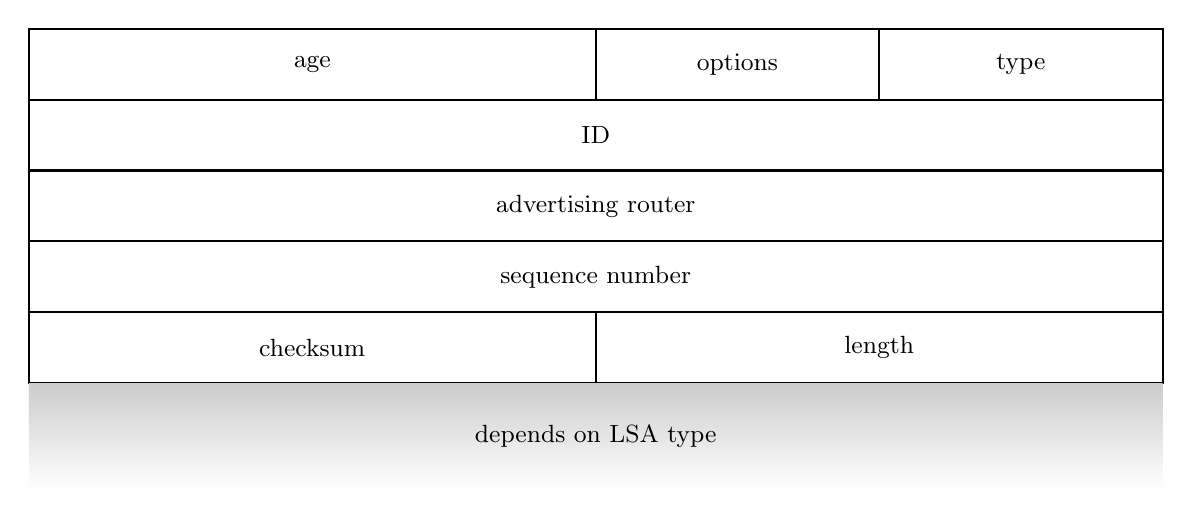
\begin{tikzpicture}
\tikzset{
    box/.style={draw,thick},
    label/.style={font=\small},
    label large/.style={},
    box label/.style={midway,font=\small,align=center},
    box label flags/.style={midway,font=\fontsize{8}{9}\selectfont,align=center},
    missing/.style={pattern=north west lines},
    length field/.style={alt=<3>{fill=red!10,very thick}},
    tos/.style={alt=<5>{fill=red!10,very thick}},
    %frag/.style={alt=<3>{fill=red!10,very thick}},
    ttl/.style={alt=<4>{fill=red!10,very thick}},
    addrs/.style={alt=<6>{fill=red!10,very thick}},
    type field/.style={alt=<2>{fill=red!10,very thick}},
    checksum/.style={alt=<6>{fill=red!10,very thick}},
}
\begin{scope}[x=0.45cm,y=0.9cm]
\draw[box] (0, 0) rectangle (16, -1)
    node[midway,label] {age};
\draw[box] (16, 0) rectangle (24, -1)
    node[midway,label] {options};
\draw[box] (24, 0) rectangle (32, -1)
    node[midway,label] {type};
\draw[box] (0, -1) rectangle (32, -2)
    node[midway,label] {ID};
\draw[box] (0, -2) rectangle (32, -3)
    node[midway,label] {advertising router};
\draw[box] (0, -3) rectangle (32, -4)
    node[midway,label] {sequence number};
\draw[box] (0, -4) rectangle (16, -5)
    node[midway,label] {checksum};
\draw[box] (16, -4) rectangle (32, -5)
    node[midway,label] {length};
\path[shading=axis,bottom color=white,top color=black!20] (0, -5) rectangle (32, -6.5)
    node[box label] {depends on LSA type};
\end{scope}
\end{tikzpicture}
\end{frame}

\begin{frame}{OSPF LSA sequences/ages}
    \begin{itemize}
    \item sequence number for getting correction version of LSAs
        \begin{itemize}
        \item some tricky rules to handle routers restarting (losing track of sequence number) and sequence number wraparound
        \end{itemize}
    \item maximum `age' for link-state advertisements
        \begin{itemize}
        \item typically minutes
        \item too-old LSAs not used for routing
        \item deliberately setting age = MaxAge used to invalidate LSAs
        \end{itemize}
    \end{itemize}
\end{frame}

\begin{frame}{OSPF LSA types}
\begin{itemize}
\item `router':
    \begin{itemize}
    \item list of links for router
    \item links = connect to other router or network
    \item links refer to ID numbers of network/router LSAs
    \item metrics for each link
    \end{itemize}
\item `network':
    \begin{itemize}
    \item list of routers for network
    \item different version of external and internal networks
    \end{itemize}
\item (later) `summary':
    \begin{itemize}
    \item part of support for \textit{areas}
    \item used when sysadmin doesn't want all routers processing whole network map
    \end{itemize}
\end{itemize}
\end{frame}

\subsection{link state database}
\begin{frame}{link-state database}
    \begin{itemize}
    \item whole collection of advertisements
    \vspace{.5cm}
    \item every router, network, link between router+network
    \item all the metrics for those
    \end{itemize}
\end{frame}


\subsection{reliable flooding}

\begin{frame}{reliable flooding (picture)}

{\small Peterson and Davie, \textit{Computer Networks: A Systems Approach}, Figure 88}
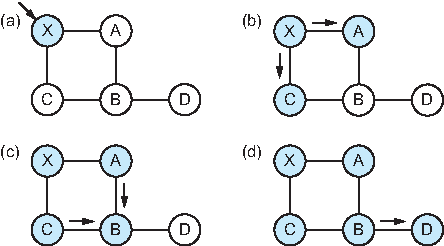
\includegraphics[width=0.8\textwidth]{../routing/sysapproach-fig88}
\end{frame}

\begin{frame}{missing from the picture}
    \begin{itemize}
    \item in picture: seems like each router directly connected to each other
    \item often we have multiple routers connected to local network
    \item can/will share link state packets by broadcasting on local network
    \end{itemize}
\end{frame}

\begin{frame}{reliable flooding in OSPF --- setup}
    \begin{itemize}
    \item for each subnetwork:
        \begin{itemize}
        \item choose a designated and backup router
        \item make sure backup becomes designated on failure
        \end{itemize}
    \item designated router will take care of propogating updates to everyone on network
    \item \ldots including waiting for acknowledgments, etc.
    \end{itemize}
\end{frame}

\begin{frame}{reliable flooding in OSPF}
    \begin{itemize}
    \item then, when receiving/generating link state packet:
    \item send to every designed+backup router of subnetwork that
        \begin{itemize}
        \item you are connected to, and
        \item you are not designated/backup router for, and
        \item you did not receive the packet from
        \end{itemize}
    \item send to every router on every subnetwork that
        \begin{itemize}
        \item you are designated router for
        \end{itemize}
    \item send = send + resend if no ACK
    \end{itemize}
\end{frame}



\subsection{shortest path first}
\usetikzlibrary{arrows.meta}
\begin{frame}{finding shortest paths}
    \begin{itemize}
    \item given full picture of network
    \item want to find all shortest paths from self 
        \begin{itemize}
        \item shortest `distance' = lowest sum of metric
        \end{itemize}
    \item only need next hop, but will compute whole path to find that
    \item assumption: everyone using shortest path
    \item usual solution: Dijkstra's algorithm
    \end{itemize}
\end{frame}



\subsection{shortest path algorithm}
\usetikzlibrary{graphs,graphs.standard,graphdrawing,quotes,positioning,matrix}
\usegdlibrary{force,layered}

\begin{frame}[fragile,label=bestFirstExample1]{Dijkstra's algorithm example 1}
\begin{tikzpicture}
\tikzset{
    graphNode/.style={draw,circle,thick,font=\tt\fontsize{9}{10}\selectfont,minimum width=.6cm,inner sep=0.2mm},
    graphEdge/.style={draw,thick},
    >=Latex,
    my graph/.style={graphs/nodes={graphNode},graphs/edges={graphEdge},graphs/edge quotes={font=\tt\small\color{blue!70!black},auto,inner sep=0.1mm}},
    my graph box/.style={}
}

\tikzset{
    my label/.style={draw=none,text width=.6cm},
    my distance/.style={text width=1cm},
    my previous/.style={text width=1cm},
    my path/.style={text width=4cm},
    my algorithm table/.style={
        tight matrix,
        nodes={font=\strut},
        row 1/.style={nodes={draw=none}},
        column 1/.style={nodes={my label}}
        column 2/.style={nodes={my distance}},
        column 3/.style={nodes={my previous}},
        column 4/.style={nodes={my path}},
        right={1cm of the graph},
    },
    hidden/.style={draw=black!50},
    hilite/.style={draw=red,font=\bfseries},
}
\tikzset{
    my label visited/.style={my label,text=black!50},
    my label updating/.style={my label,font=\bfseries,text=red},
    my label changed/.style={my label,font=\bfseries,text=blue!50!black},
    my label unvisited/.style={my label},
    my distance visited/.style={black!50},
    my distance updating/.style={},
    my distance changed/.style={red},
    my distance unvisited/.style={},
    my previous visited/.style={},
    my previous updating/.style={},
    my previous changed/.style={red},
    my previous unvisited/.style={},
    my path visited/.style={},
    my path updating/.style={},
    my path changed/.style={red},
    my path unvisited/.style={},
}
% FIXME: hilite overwriting examples
    
\tikzset{graph at A/.style={},edges from A/.style={},
graph at B/.style={},edges from B/.style={},
graph at C/.style={},edges from C/.style={},
graph at D/.style={},edges from D/.style={},
graph at E/.style={},edges from E/.style={},
graph at F/.style={},edges from F/.style={},
graph at G/.style={},edges from G/.style={},}

\tikzset{
    alt=<1>{}{},
}

\tikzset{
    alt=<2>{graph at A/.style={hilite},edges from A/.style={hilite},}{},
}

\tikzset{
    alt=<3>{graph at A/.style={hidden},graph at D/.style={hilite},edges from D/.style={hilite},}{},
}

\tikzset{
    alt=<4>{graph at A/.style={hidden},graph at C/.style={hilite},edges from C/.style={hilite},graph at D/.style={hidden},}{},
}

\tikzset{
    alt=<5>{graph at A/.style={hidden},graph at C/.style={hidden},graph at D/.style={hidden},graph at E/.style={hilite},edges from E/.style={hilite},}{},
}

\tikzset{
    alt=<6>{graph at A/.style={hidden},graph at B/.style={hilite},edges from B/.style={hilite},graph at C/.style={hidden},graph at D/.style={hidden},graph at E/.style={hidden},}{},
}

\tikzset{
    alt=<7>{graph at A/.style={hidden},graph at B/.style={hidden},graph at C/.style={hidden},graph at D/.style={hidden},graph at E/.style={hidden},graph at F/.style={hilite},edges from F/.style={hilite},}{},
}

\tikzset{
    alt=<8>{graph at A/.style={hidden},graph at B/.style={hidden},graph at C/.style={hidden},graph at D/.style={hidden},graph at E/.style={hidden},graph at F/.style={hidden},graph at G/.style={hilite},edges from G/.style={hilite},}{},
}

\matrix[my graph box] (the graph) {
\begin{scope}[my graph]
\graph[spring layout]{
    A[graph at A] ->[edges from A,edges from A,"2"] C[graph at C],
A[graph at A] ->[edges from A,edges from A,"1"] D[graph at D],

B[graph at B] ->[edges from B,edges from B,"2"] A[graph at A],

C[graph at C] ->[edges from C,edges from C,"1"] D[graph at D],
C[graph at C] ->[edges from C,edges from C,"2"] F[graph at F],

D[graph at D] ->[edges from D,edges from D,"5"] B[graph at B],
D[graph at D] ->[edges from D,edges from D,"1"] E[graph at E],
D[graph at D] ->[edges from D,edges from D,"6"] F[graph at F],
D[graph at D] ->[edges from D,edges from D,"5"] G[graph at G],

E[graph at E] ->[edges from E,edges from E,"1"] B[graph at B],

F[graph at F] ->[edges from F,edges from F,"10"] G[graph at G],

G[graph at G] ->[edges from G,edges from G,"3"] E[graph at E],

};
\end{scope}
\\
};

\begin{onlyenv}<1>
\matrix[
    my algorithm table,
    ] (the table) {
~ \& dist \& prev \& path \\
|[my label unvisited]| A \& |[my distance unvisited]| 0\& |[my previous unvisited]| --- \& |[my path unvisited]| A\\
|[my label unvisited]| B \& |[my distance unvisited]| $\infty$\& |[my previous unvisited]| --- \& |[my path unvisited]| ---\\
|[my label unvisited]| C \& |[my distance unvisited]| $\infty$\& |[my previous unvisited]| --- \& |[my path unvisited]| ---\\
|[my label unvisited]| D \& |[my distance unvisited]| $\infty$\& |[my previous unvisited]| --- \& |[my path unvisited]| ---\\
|[my label unvisited]| E \& |[my distance unvisited]| $\infty$\& |[my previous unvisited]| --- \& |[my path unvisited]| ---\\
|[my label unvisited]| F \& |[my distance unvisited]| $\infty$\& |[my previous unvisited]| --- \& |[my path unvisited]| ---\\
|[my label unvisited]| G \& |[my distance unvisited]| $\infty$\& |[my previous unvisited]| --- \& |[my path unvisited]| ---\\
};
\end{onlyenv}
            
\begin{onlyenv}<2>
\matrix[
    my algorithm table,
    ] (the table) {
~ \& dist \& prev \& path \\
|[my label updating]| A \& |[my distance updating]| 0\& |[my previous updating]| --- \& |[my path updating]| A\\
|[my label unvisited]| B \& |[my distance unvisited]| $\infty$\& |[my previous unvisited]| --- \& |[my path unvisited]| ---\\
|[my label changed]| C \& |[my distance changed]| 2\& |[my previous changed]| A \& |[my path changed]| A$\rightarrow$C\\
|[my label changed]| D \& |[my distance changed]| 1\& |[my previous changed]| A \& |[my path changed]| A$\rightarrow$D\\
|[my label unvisited]| E \& |[my distance unvisited]| $\infty$\& |[my previous unvisited]| --- \& |[my path unvisited]| ---\\
|[my label unvisited]| F \& |[my distance unvisited]| $\infty$\& |[my previous unvisited]| --- \& |[my path unvisited]| ---\\
|[my label unvisited]| G \& |[my distance unvisited]| $\infty$\& |[my previous unvisited]| --- \& |[my path unvisited]| ---\\
};
\end{onlyenv}
            
\begin{onlyenv}<3>
\matrix[
    my algorithm table,
    ] (the table) {
~ \& dist \& prev \& path \\
|[my label visited]| A \& |[my distance visited]| 0\& |[my previous visited]| --- \& |[my path visited]| A\\
|[my label changed]| B \& |[my distance changed]| 6\& |[my previous changed]| D \& |[my path changed]| A$\rightarrow$D$\rightarrow$B\\
|[my label unvisited]| C \& |[my distance unvisited]| 2\& |[my previous unvisited]| A \& |[my path unvisited]| A$\rightarrow$C\\
|[my label updating]| D \& |[my distance updating]| 1\& |[my previous updating]| A \& |[my path updating]| A$\rightarrow$D\\
|[my label changed]| E \& |[my distance changed]| 2\& |[my previous changed]| D \& |[my path changed]| A$\rightarrow$D$\rightarrow$E\\
|[my label changed]| F \& |[my distance changed]| 7\& |[my previous changed]| D \& |[my path changed]| A$\rightarrow$D$\rightarrow$F\\
|[my label changed]| G \& |[my distance changed]| 6\& |[my previous changed]| D \& |[my path changed]| A$\rightarrow$D$\rightarrow$G\\
};
\end{onlyenv}
            
\begin{onlyenv}<4>
\matrix[
    my algorithm table,
    ] (the table) {
~ \& dist \& prev \& path \\
|[my label visited]| A \& |[my distance visited]| 0\& |[my previous visited]| --- \& |[my path visited]| A\\
|[my label unvisited]| B \& |[my distance unvisited]| 6\& |[my previous unvisited]| D \& |[my path unvisited]| A$\rightarrow$D$\rightarrow$B\\
|[my label updating]| C \& |[my distance updating]| 2\& |[my previous updating]| A \& |[my path updating]| A$\rightarrow$C\\
|[my label visited]| D \& |[my distance visited]| 1\& |[my previous visited]| A \& |[my path visited]| A$\rightarrow$D\\
|[my label unvisited]| E \& |[my distance unvisited]| 2\& |[my previous unvisited]| D \& |[my path unvisited]| A$\rightarrow$D$\rightarrow$E\\
|[my label changed]| F \& |[my distance changed]| 4\& |[my previous changed]| C \& |[my path changed]| A$\rightarrow$C$\rightarrow$F\\
|[my label unvisited]| G \& |[my distance unvisited]| 6\& |[my previous unvisited]| D \& |[my path unvisited]| A$\rightarrow$D$\rightarrow$G\\
};
\end{onlyenv}
            
\begin{onlyenv}<5>
\matrix[
    my algorithm table,
    ] (the table) {
~ \& dist \& prev \& path \\
|[my label visited]| A \& |[my distance visited]| 0\& |[my previous visited]| --- \& |[my path visited]| A\\
|[my label changed]| B \& |[my distance changed]| 3\& |[my previous changed]| E \& |[my path changed]| A$\rightarrow$D$\rightarrow$E$\rightarrow$B\\
|[my label visited]| C \& |[my distance visited]| 2\& |[my previous visited]| A \& |[my path visited]| A$\rightarrow$C\\
|[my label visited]| D \& |[my distance visited]| 1\& |[my previous visited]| A \& |[my path visited]| A$\rightarrow$D\\
|[my label updating]| E \& |[my distance updating]| 2\& |[my previous updating]| D \& |[my path updating]| A$\rightarrow$D$\rightarrow$E\\
|[my label unvisited]| F \& |[my distance unvisited]| 4\& |[my previous unvisited]| C \& |[my path unvisited]| A$\rightarrow$C$\rightarrow$F\\
|[my label unvisited]| G \& |[my distance unvisited]| 6\& |[my previous unvisited]| D \& |[my path unvisited]| A$\rightarrow$D$\rightarrow$G\\
};
\end{onlyenv}
            
\begin{onlyenv}<6>
\matrix[
    my algorithm table,
    ] (the table) {
~ \& dist \& prev \& path \\
|[my label visited]| A \& |[my distance visited]| 0\& |[my previous visited]| --- \& |[my path visited]| A\\
|[my label updating]| B \& |[my distance updating]| 3\& |[my previous updating]| E \& |[my path updating]| A$\rightarrow$D$\rightarrow$E$\rightarrow$B\\
|[my label visited]| C \& |[my distance visited]| 2\& |[my previous visited]| A \& |[my path visited]| A$\rightarrow$C\\
|[my label visited]| D \& |[my distance visited]| 1\& |[my previous visited]| A \& |[my path visited]| A$\rightarrow$D\\
|[my label visited]| E \& |[my distance visited]| 2\& |[my previous visited]| D \& |[my path visited]| A$\rightarrow$D$\rightarrow$E\\
|[my label unvisited]| F \& |[my distance unvisited]| 4\& |[my previous unvisited]| C \& |[my path unvisited]| A$\rightarrow$C$\rightarrow$F\\
|[my label unvisited]| G \& |[my distance unvisited]| 6\& |[my previous unvisited]| D \& |[my path unvisited]| A$\rightarrow$D$\rightarrow$G\\
};
\end{onlyenv}
            
\begin{onlyenv}<7>
\matrix[
    my algorithm table,
    ] (the table) {
~ \& dist \& prev \& path \\
|[my label visited]| A \& |[my distance visited]| 0\& |[my previous visited]| --- \& |[my path visited]| A\\
|[my label visited]| B \& |[my distance visited]| 3\& |[my previous visited]| E \& |[my path visited]| A$\rightarrow$D$\rightarrow$E$\rightarrow$B\\
|[my label visited]| C \& |[my distance visited]| 2\& |[my previous visited]| A \& |[my path visited]| A$\rightarrow$C\\
|[my label visited]| D \& |[my distance visited]| 1\& |[my previous visited]| A \& |[my path visited]| A$\rightarrow$D\\
|[my label visited]| E \& |[my distance visited]| 2\& |[my previous visited]| D \& |[my path visited]| A$\rightarrow$D$\rightarrow$E\\
|[my label updating]| F \& |[my distance updating]| 4\& |[my previous updating]| C \& |[my path updating]| A$\rightarrow$C$\rightarrow$F\\
|[my label unvisited]| G \& |[my distance unvisited]| 6\& |[my previous unvisited]| D \& |[my path unvisited]| A$\rightarrow$D$\rightarrow$G\\
};
\end{onlyenv}
            
\begin{onlyenv}<8>
\matrix[
    my algorithm table,
    ] (the table) {
~ \& dist \& prev \& path \\
|[my label visited]| A \& |[my distance visited]| 0\& |[my previous visited]| --- \& |[my path visited]| A\\
|[my label visited]| B \& |[my distance visited]| 3\& |[my previous visited]| E \& |[my path visited]| A$\rightarrow$D$\rightarrow$E$\rightarrow$B\\
|[my label visited]| C \& |[my distance visited]| 2\& |[my previous visited]| A \& |[my path visited]| A$\rightarrow$C\\
|[my label visited]| D \& |[my distance visited]| 1\& |[my previous visited]| A \& |[my path visited]| A$\rightarrow$D\\
|[my label visited]| E \& |[my distance visited]| 2\& |[my previous visited]| D \& |[my path visited]| A$\rightarrow$D$\rightarrow$E\\
|[my label visited]| F \& |[my distance visited]| 4\& |[my previous visited]| C \& |[my path visited]| A$\rightarrow$C$\rightarrow$F\\
|[my label updating]| G \& |[my distance updating]| 6\& |[my previous updating]| D \& |[my path updating]| A$\rightarrow$D$\rightarrow$G\\
};
\end{onlyenv}
            


\begin{visibleenv}<4>
\draw[<-,very thick] (the table-5-2.north) -- ++(2cm,3cm) node[draw,thick,align=left,fill=white] {
    D is adjacent --- \\ but not a shorter path
};
\draw[<-,very thick] (the table-7-2.south) -- ++(1cm,-2cm) node[fill=white,draw,thick,align=left] {
    F updated from distance 7 (via D) \\ to distance 4 (via C)
};
\end{visibleenv}

\end{tikzpicture}
\end{frame}

\begin{frame}[fragile,label=bestFirstExample2]{Dijkstra's algorithm example 2}
\begin{tikzpicture}
\tikzset{
    graphNode/.style={draw,circle,thick,font=\tt\fontsize{9}{10}\selectfont,minimum width=.6cm,inner sep=0.2mm},
    graphEdge/.style={draw,thick},
    >=Latex,
    my graph/.style={graphs/nodes={graphNode},graphs/edges={graphEdge},graphs/edge quotes={font=\tt\small\color{blue!70!black},auto,inner sep=0.1mm},graphs/node distance={2cm}},
    my graph box/.style={}
}

\tikzset{
    my label/.style={draw=none,text width=.6cm},
    my distance/.style={text width=1cm},
    my previous/.style={text width=1cm},
    my path/.style={text width=4cm},
    my algorithm table/.style={
        tight matrix,
        nodes={font=\strut},
        row 1/.style={nodes={draw=none}},
        column 1/.style={nodes={my label}}
        column 2/.style={nodes={my distance}},
        column 3/.style={nodes={my previous}},
        column 4/.style={nodes={my path}},
        right={1cm of the graph},
    },
    hidden/.style={draw=black!50},
    hilite/.style={draw=red,font=\bfseries},
}
\tikzset{
    my label visited/.style={my label,text=black!50},
    my label updating/.style={my label,font=\bfseries,text=red},
    my label changed/.style={my label,font=\bfseries,text=blue!50!black},
    my label unvisited/.style={my label},
    my distance visited/.style={black!50},
    my distance updating/.style={},
    my distance changed/.style={red},
    my distance unvisited/.style={},
    my previous visited/.style={},
    my previous updating/.style={},
    my previous changed/.style={red},
    my previous unvisited/.style={},
    my path visited/.style={},
    my path updating/.style={},
    my path changed/.style={red},
    my path unvisited/.style={},
}
% FIXME: hilite overwriting examples
    
\tikzset{graph at A/.style={},edges from A/.style={},
graph at B/.style={},edges from B/.style={},
graph at C/.style={},edges from C/.style={},
graph at D/.style={},edges from D/.style={},
graph at E/.style={},edges from E/.style={},
graph at G/.style={},edges from G/.style={},}

\tikzset{
    alt=<1>{}{},
}

\tikzset{
    alt=<2>{graph at A/.style={hilite},edges from A/.style={hilite},}{},
}

\tikzset{
    alt=<3>{graph at A/.style={hidden},graph at B/.style={hilite},edges from B/.style={hilite},}{},
}

\tikzset{
    alt=<4>{graph at A/.style={hidden},graph at B/.style={hidden},graph at C/.style={hilite},edges from C/.style={hilite},}{},
}

\tikzset{
    alt=<5>{graph at A/.style={hidden},graph at B/.style={hidden},graph at C/.style={hidden},graph at G/.style={hilite},edges from G/.style={hilite},}{},
}

\tikzset{
    alt=<6>{graph at A/.style={hidden},graph at B/.style={hidden},graph at C/.style={hidden},graph at D/.style={hilite},edges from D/.style={hilite},graph at G/.style={hidden},}{},
}

\tikzset{
    alt=<7>{graph at A/.style={hidden},graph at B/.style={hidden},graph at C/.style={hidden},graph at D/.style={hidden},graph at E/.style={hilite},edges from E/.style={hilite},graph at G/.style={hidden},}{},
}

\matrix[my graph box] (the graph) {
\begin{scope}[my graph]
\graph[spring layout]{
    A[graph at A] --[edges from A,edges from B,"7"] B[graph at B],
A[graph at A] --[edges from A,edges from C,"9"] C[graph at C],
A[graph at A] --[edges from A,edges from G,"14"] G[graph at G],

B[graph at B] --[edges from B,edges from C,"10"'] C[graph at C],
B[graph at B] --[edges from B,edges from D,"15"] D[graph at D],

C[graph at C] --[edges from C,edges from D,"11"] D[graph at D],
C[graph at C] --[edges from C,edges from G,"2"] G[graph at G],

D[graph at D] --[edges from D,edges from E,"6"] E[graph at E],

E[graph at E] --[edges from E,edges from G,"9"] G[graph at G],


};
\end{scope}
\\
};

\begin{onlyenv}<1>
\matrix[
    my algorithm table,
    ] (the table) {
~ \& dist \& prev \& path \\
|[my label unvisited]| A \& |[my distance unvisited]| 0\& |[my previous unvisited]| --- \& |[my path unvisited]| A\\
|[my label unvisited]| B \& |[my distance unvisited]| $\infty$\& |[my previous unvisited]| --- \& |[my path unvisited]| ---\\
|[my label unvisited]| C \& |[my distance unvisited]| $\infty$\& |[my previous unvisited]| --- \& |[my path unvisited]| ---\\
|[my label unvisited]| D \& |[my distance unvisited]| $\infty$\& |[my previous unvisited]| --- \& |[my path unvisited]| ---\\
|[my label unvisited]| E \& |[my distance unvisited]| $\infty$\& |[my previous unvisited]| --- \& |[my path unvisited]| ---\\
|[my label unvisited]| G \& |[my distance unvisited]| $\infty$\& |[my previous unvisited]| --- \& |[my path unvisited]| ---\\
};
\end{onlyenv}
            
\begin{onlyenv}<2>
\matrix[
    my algorithm table,
    ] (the table) {
~ \& dist \& prev \& path \\
|[my label updating]| A \& |[my distance updating]| 0\& |[my previous updating]| --- \& |[my path updating]| A\\
|[my label changed]| B \& |[my distance changed]| 7\& |[my previous changed]| A \& |[my path changed]| A$\rightarrow$B\\
|[my label changed]| C \& |[my distance changed]| 9\& |[my previous changed]| A \& |[my path changed]| A$\rightarrow$C\\
|[my label unvisited]| D \& |[my distance unvisited]| $\infty$\& |[my previous unvisited]| --- \& |[my path unvisited]| ---\\
|[my label unvisited]| E \& |[my distance unvisited]| $\infty$\& |[my previous unvisited]| --- \& |[my path unvisited]| ---\\
|[my label changed]| G \& |[my distance changed]| 14\& |[my previous changed]| A \& |[my path changed]| A$\rightarrow$G\\
};
\end{onlyenv}
            
\begin{onlyenv}<3>
\matrix[
    my algorithm table,
    ] (the table) {
~ \& dist \& prev \& path \\
|[my label visited]| A \& |[my distance visited]| 0\& |[my previous visited]| --- \& |[my path visited]| A\\
|[my label updating]| B \& |[my distance updating]| 7\& |[my previous updating]| A \& |[my path updating]| A$\rightarrow$B\\
|[my label unvisited]| C \& |[my distance unvisited]| 9\& |[my previous unvisited]| A \& |[my path unvisited]| A$\rightarrow$C\\
|[my label changed]| D \& |[my distance changed]| 22\& |[my previous changed]| B \& |[my path changed]| A$\rightarrow$B$\rightarrow$D\\
|[my label unvisited]| E \& |[my distance unvisited]| $\infty$\& |[my previous unvisited]| --- \& |[my path unvisited]| ---\\
|[my label unvisited]| G \& |[my distance unvisited]| 14\& |[my previous unvisited]| A \& |[my path unvisited]| A$\rightarrow$G\\
};
\end{onlyenv}
            
\begin{onlyenv}<4>
\matrix[
    my algorithm table,
    ] (the table) {
~ \& dist \& prev \& path \\
|[my label visited]| A \& |[my distance visited]| 0\& |[my previous visited]| --- \& |[my path visited]| A\\
|[my label visited]| B \& |[my distance visited]| 7\& |[my previous visited]| A \& |[my path visited]| A$\rightarrow$B\\
|[my label updating]| C \& |[my distance updating]| 9\& |[my previous updating]| A \& |[my path updating]| A$\rightarrow$C\\
|[my label changed]| D \& |[my distance changed]| 20\& |[my previous changed]| C \& |[my path changed]| A$\rightarrow$C$\rightarrow$D\\
|[my label unvisited]| E \& |[my distance unvisited]| $\infty$\& |[my previous unvisited]| --- \& |[my path unvisited]| ---\\
|[my label changed]| G \& |[my distance changed]| 11\& |[my previous changed]| C \& |[my path changed]| A$\rightarrow$C$\rightarrow$G\\
};
\end{onlyenv}
            
\begin{onlyenv}<5>
\matrix[
    my algorithm table,
    ] (the table) {
~ \& dist \& prev \& path \\
|[my label visited]| A \& |[my distance visited]| 0\& |[my previous visited]| --- \& |[my path visited]| A\\
|[my label visited]| B \& |[my distance visited]| 7\& |[my previous visited]| A \& |[my path visited]| A$\rightarrow$B\\
|[my label visited]| C \& |[my distance visited]| 9\& |[my previous visited]| A \& |[my path visited]| A$\rightarrow$C\\
|[my label unvisited]| D \& |[my distance unvisited]| 20\& |[my previous unvisited]| C \& |[my path unvisited]| A$\rightarrow$C$\rightarrow$D\\
|[my label changed]| E \& |[my distance changed]| 20\& |[my previous changed]| G \& |[my path changed]| A$\rightarrow$C$\rightarrow$G$\rightarrow$E\\
|[my label updating]| G \& |[my distance updating]| 11\& |[my previous updating]| C \& |[my path updating]| A$\rightarrow$C$\rightarrow$G\\
};
\end{onlyenv}
            
\begin{onlyenv}<6>
\matrix[
    my algorithm table,
    ] (the table) {
~ \& dist \& prev \& path \\
|[my label visited]| A \& |[my distance visited]| 0\& |[my previous visited]| --- \& |[my path visited]| A\\
|[my label visited]| B \& |[my distance visited]| 7\& |[my previous visited]| A \& |[my path visited]| A$\rightarrow$B\\
|[my label visited]| C \& |[my distance visited]| 9\& |[my previous visited]| A \& |[my path visited]| A$\rightarrow$C\\
|[my label updating]| D \& |[my distance updating]| 20\& |[my previous updating]| C \& |[my path updating]| A$\rightarrow$C$\rightarrow$D\\
|[my label unvisited]| E \& |[my distance unvisited]| 20\& |[my previous unvisited]| G \& |[my path unvisited]| A$\rightarrow$C$\rightarrow$G$\rightarrow$E\\
|[my label visited]| G \& |[my distance visited]| 11\& |[my previous visited]| C \& |[my path visited]| A$\rightarrow$C$\rightarrow$G\\
};
\end{onlyenv}
            
\begin{onlyenv}<7>
\matrix[
    my algorithm table,
    ] (the table) {
~ \& dist \& prev \& path \\
|[my label visited]| A \& |[my distance visited]| 0\& |[my previous visited]| --- \& |[my path visited]| A\\
|[my label visited]| B \& |[my distance visited]| 7\& |[my previous visited]| A \& |[my path visited]| A$\rightarrow$B\\
|[my label visited]| C \& |[my distance visited]| 9\& |[my previous visited]| A \& |[my path visited]| A$\rightarrow$C\\
|[my label visited]| D \& |[my distance visited]| 20\& |[my previous visited]| C \& |[my path visited]| A$\rightarrow$C$\rightarrow$D\\
|[my label updating]| E \& |[my distance updating]| 20\& |[my previous updating]| G \& |[my path updating]| A$\rightarrow$C$\rightarrow$G$\rightarrow$E\\
|[my label visited]| G \& |[my distance visited]| 11\& |[my previous visited]| C \& |[my path visited]| A$\rightarrow$C$\rightarrow$G\\
};
\end{onlyenv}
            


\end{tikzpicture}
\end{frame}


\subsection{shortest path consistency}
\begin{frame}{consistency}
\begin{tikzpicture}
\tikzset{mynode/.style={draw,circle,very thick}}
\node[mynode] (A) at (0,0) {A};
\node[mynode] (B) at (4,0) {B};
\node[mynode] (low1) at (3,-2) {~};
\node[mynode] (low2) at (6,-2) {~};
\node[mynode] (C) at (8,0) {C};
\node[mynode] (high1) at (6,1) {~};
\tikzset{myedge/.style={draw,ultra thick}}
\path[myedge] (A) -- (B);
\path[myedge] (A) -- (low1);
\path[myedge] (low1) -- (low2);
\path[myedge] (low2) -- (C);
\path[myedge] (B) -- (high1);
\path[myedge] (high1) -- (C);
\path[very thick,dotted,red,-Latex] (A) .. controls (4, -3) .. (C);
\path[very thick,violet,-Latex] (A) -- (B);
\end{tikzpicture}
\begin{itemize}
\item if A sends packet for C to B, how does A know B won't send it back?
\vspace{.5cm}
\item hope: if A thought shortest path to C was through B, then B should agree
\item problem: not always true
\end{itemize}
\end{frame}

\begin{frame}[fragile]{inconsistency}
\begin{tikzpicture}
\tikzset{
    mynode/.style={draw,circle,very thick},
    myedge/.style={draw,ultra thick},
    computer/.style={inner sep=0mm,outer sep=0mm,execute at begin node={\computer}},
    switch/.style={inner sep=0mm,outer sep=0mm,execute at begin node={\switch}},
    port/.style={pos=0.95,fill=white,circle,draw,inner sep=0mm},
    port beginning/.style={pos=0.05,fill=white,circle,draw,inner sep=0mm},
    route table/.style={
        matrix of nodes,ampersand replacement=\&,
        column 1/.style={nodes={draw,thick,text width=2.5cm,font=\tiny\tt,text depth=0mm,minimum height=0.5cm,inner sep=1mm}},
        column 2/.style={nodes={draw,thick,text width=.5cm,font=\small\tt,text depth=0mm,minimum height=0.5cm,inner sep=1mm}},
        row 1/.style={nodes={draw=none,font=\small}},
    },
    mac label/.style={
        draw,fill=white,inner sep=1mm,font=\tiny\tt,
    },
    n real/.style={solid},
    n real at/.style={alt=<#1->{solid},alt=<#1>{fill=red!10}},
    n real until/.style={alt=<1-#1>{solid}},
    tn/.style={draw,dotted,circle,very thick},
    real at/.style={alt=<#1->{solid},alt=<#1>{fill=red!10}},
    connect/.style={draw,very thick,-Latex},
    connect big/.style={draw,ultra thick,-Latex},
    actual at/.style={alt=<#1->{draw=red,solid},alt=<#1>{draw,solid}},
    consider at/.style={alt=<#1>{draw=red}},
    msg link/.style={draw,violet,line width=1.2mm,-Latex},
    msg data/.style={draw=violet,line width=1mm,fill=white,align=left},
    explain box/.style={draw,ultra thick,draw=red,text=black,anchor=north,at={(4, -4)}, align=left},
}
\node[mynode] (A) at (0,0) {A};
\node[mynode] (B) at (4,0) {B};
\node[mynode] (low1) at (3,-2) {~};
\node[mynode] (low2) at (6,-2) {~};
\node[mynode] (C) at (8,0) {C};
\node[mynode] (high1) at (6,1) {~};
\path[myedge] (A) -- (B);
\path[myedge] (A) -- (low1);
\path[myedge] (low1) -- (low2);
\path[myedge] (low2) -- (C);
\path[myedge] (B) -- (high1);
\path[myedge] (high1) -- (C) node[midway,font=\huge,text=red,draw=none]{X};
\begin{visibleenv}<2->
    \path[msg link] (high1) -- (B);
    \path[msg link] (C) -- (low2);
    \node[explain box] {B thinks best route to C: through A \\ A thinks best route to C: through B};
\end{visibleenv}
%\path[very thick,dotted,red,-Latex] (A) .. controls (4, -3) .. (C);
%\path[very thick,dotted,red,-Latex] (A) -- (B);
\end{tikzpicture}
\end{frame}

\begin{frame}{temporary bad routes}
    \begin{itemize}
    \item while waiting for link state updates to propogate
    \item can have too-slow routes
    \item can have routing loops
    \vspace{.5cm}
    \item hope: this is only a few seconds at most
        \begin{itemize}
        \item and routing loop doesn't cause huge explosion of traffic
        \end{itemize}
    \end{itemize}
\end{frame}


\subsection{convergence}
\usetikzlibrary{calc,shapes.misc}
\begin{frame}{convergence time}
\begin{tikzpicture}
\tikzset{
    mynode/.style={draw,circle,very thick,font=\small},
    myedge/.style={draw,ultra thick},
}
\node[mynode] (A) at (0,0) {A};
\node[mynode] (B) at (4,0) {B};
\node[mynode] (C) at (8,0) {C};
\node[mynode] (D) at (8,-4) {D};
\node[mynode] (E) at (4,-4) {E};
\node[mynode] (F) at (0,-4) {F};
\foreach \x/\y in {A/B,B/C,C/D,D/E,E/F,F/A} {
    \draw[myedge] (\x) -- (\y);
}
\begin{visibleenv}<2>
    \node[draw,red,very thick,cross out] at ($(A)!0.5!(B)$) {};
\end{visibleenv}
\end{tikzpicture}
\begin{itemize}
\item exercise: how many steps to fix A's next hop for B, C, D, etc.\ldots
    \begin{itemize}
    \item with distance vector?
    \item with link state?
    \end{itemize}
\end{itemize}
\end{frame}


\subsection{networks versus routers}
\usetikzlibrary{fit,matrix}
\usetikzlibrary{arrows.meta,calc,shapes}
\providecommand{\computer}{%
    
\includegraphics[width=0.7cm]{../common/Noun_project_216.pdf}
}
\providecommand{\computerAlt}{%
    
\includegraphics[width=0.8cm]{../common/Noun_project_alt_cpu.pdf}
}
\providecommand{\switch}{%
    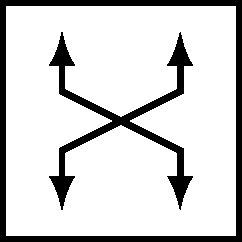
\includegraphics[width=0.8cm]{../common/fig-switch.pdf}
}
\providecommand{\router}{%
    
\includegraphics[width=0.8cm]{../common/fig-router.pdf}
}

\begin{frame}[fragile]{networks v routers (LS)}
\tikzset{
    mynode/.style={draw,circle,very thick,font=\small},
    myedge/.style={draw,ultra thick},
    computer/.style={inner sep=0mm,outer sep=0mm,execute at begin node={\computer}},
    switch/.style={inner sep=0mm,outer sep=0mm,execute at begin node={\switch}},
    router/.style={inner sep=0mm,outer sep=0mm,execute at begin node={\router}},
    port/.style={pos=0.95,fill=white,circle,draw,inner sep=0mm},
    port beginning/.style={pos=0.05,fill=white,circle,draw,inner sep=0mm},
    connect/.style={draw,thick,Latex-Latex},
    msg link/.style={draw,violet,line width=1.2mm,-Latex},
    msg data/.style={draw=violet,line width=0.8mm,fill=white,align=left,font=\fontsize{9}{10}\selectfont,align=left},
}
\begin{tikzpicture}
\foreach \x/\offX/\offY in {1/0/0,2/3/0} {
    \begin{scope}[xshift=\offX cm,yshift=\offY cm]
    \node[computer] (c\x-a) at (0, 0) {};
    \node[computer] (c\x-b) at (1, 0) {};
    \node[switch] (s\x) at (0.5, -1) {};
    \draw[connect] (c\x-a) -- (s\x);
    \draw[connect] (c\x-b) -- (s\x);
    \end{scope}
}
\foreach \x/\offX/\offY in {3/0/-6} {
    \begin{scope}[xshift=\offX cm,yshift=\offY cm]
    \node[computer] (c\x-a) at (0, 0) {};
    \node[computer] (c\x-b) at (1, -.5) {};
    \node[computer] (c\x-c) at (2, -.5) {};
    \node[switch] (s\x) at (0.5, 2) {};
    \node[switch] (s\x-b) at (1.5, 1) {};
    \draw[connect] (c\x-a) -- (s\x);
    \draw[connect] (c\x-b) -- (s\x-b);
    \draw[connect] (c\x-c) -- (s\x-b);
    \draw[connect] (s\x) -- (s\x-b);
    \end{scope}
}
\node[switch] (s4) at (4, -5) {};
\node[router,label={south:R1}] (r1) at (-1, -3) {};
\node[router,label={south:R2}] (r2) at (2, -2) {};
\node[router,label={south:R3}] (r3) at (2, -3.4) {};
\node[router,label={south:R4}] (r4) at (5, -3.25) {};
\foreach \x/\y in {r1/s1,r2/s1,r2/s2,r3/s3,r2/s4,r1/s3,r3/s4,s3/r3,s2/r4,r4/s4} {
    \draw[connect] (\x) -- (\y);
}
\draw[connect,alt=<4>{red}] (r1) -- (r2);
\begin{visibleenv}<2->
\draw[dotted, very thick,fill=green,fill opacity=0.1,text opacity=1.] ([xshift=-.2cm]c1-a.north west) -- ([xshift=.2cm]c1-b.north east)
    node[midway,above] {N1}
    -- ([xshift=.1cm]r2.west) -- ([xshift=-.1cm]r1.north east) -- cycle;
\draw[dotted, very thick,fill=violet,fill opacity=0.1,text opacity=1.] ([xshift=-.2cm]c2-a.north west) -- ([xshift=.2cm]c2-b.north east)
    node[midway,above] {N2}
    -- ([xshift=.1cm]r4.north east) -- ([xshift=-.1cm]r2.east) -- cycle;
\draw[dotted, very thick,fill=yellow,fill opacity=0.1,text opacity=1.] ([xshift=-.2cm]c3-a.south west) -- ([xshift=-.2cm]c3-b.south west) -- ([xshift=.2cm]c3-c.south east)
    -- (s3-b.north east) -- (r3.west) -- (r1.east) node[midway] {N3} -- cycle;
\draw[dotted, very thick,fill=red,fill opacity=0.1,text opacity=1.] (r2.south east) -- (r4.south west) node[midway]{N4}
    -- (s4.south east) -- (s4.south west) -- (r3.south east) -- cycle;
    -- (s3-b.north east) -- (r3.west) -- (r1.east) node[midway,yshift=-.5cm] {N3} -- cycle;
\end{visibleenv}

\begin{visibleenv}<3->
\begin{scope}[xshift=8cm]
\node[mynode] (R1r) at (0, 0) {R1};
\node[mynode] (N1r) at (2, 1) {N1};
\node[mynode] (R2r) at (4, 0) {R2};
\node[mynode] (N2r) at (4, -2) {N2};
\node[mynode] (R3r) at (0, -4) {R3};
\node[mynode] (N3r) at (0, -2) {N3};
\node[mynode] (N4r) at (2, -2) {N4};
\node[mynode] (R4r) at (4, -4) {R4};
\draw[connect,alt=<4>{red}] (R1r) -- (R2r);
\draw[connect] (R1r) -- (N1r);
\draw[connect] (R2r) -- (N1r);
\draw[connect] (R1r) -- (N3r);
\draw[connect] (R3r) -- (N3r);
\draw[connect] (R3r) -- (N4r);
\draw[connect] (R4r) -- (N4r);
\draw[connect] (R2r) -- (N4r);
\draw[connect] (R2r) -- (N2r);
\draw[connect] (R4r) -- (N2r);
    \begin{visibleenv}<3>
    \node[anchor=north,draw=red, ultra thick] at (2, -5) {
        graph has nodes for routers+networks
    };
    \end{visibleenv}
    \begin{visibleenv}<4>
    \node[anchor=north,draw=red, ultra thick] at (2, -5) {
        can have direct router-router link
    };
    \end{visibleenv}
\end{scope}
\end{visibleenv}
\end{tikzpicture}
\end{frame}
 

\section{multipath/load balancing}
\begin{frame}[fragile]{two good choices?}
\begin{tikzpicture}
\tikzset{
    n/.style={draw,circle,very thick},
    connect/.style={draw,very thick,Latex-Latex},
}
\node[n] (A) at (0, 0) {A};
\node[n] (B) at (3, -2) {B};
\node[n] (D) at (6, -2) {D};
\node[n] (F) at (9, -2) {F};
\node[n] (C) at (3, 2) {C};
\node[n] (E) at (6, 2) {E};
\node[n] (G) at (9, 2) {G};
\node[n] (H) at (12, 0) {H};
\foreach \x/\y in {A/B,B/D,D/F,F/H,A/C,C/E,E/G,G/H} {
    \draw[connect] (\x) -- (\y);
}
\draw[ultra thick,red,dotted,-Latex] (A) .. controls (3, -4) .. (6, -4) .. controls (9, -4) .. (H);
\draw[ultra thick,red,dotted,-Latex] (A) .. controls (3, 4) .. (6, 4) .. controls (9, 4) .. (H);
\end{tikzpicture}
\end{frame}

\begin{frame}{splitting packets}
    \begin{itemize}
    \item na\"ive idea: send every other packet on bottom link
    \vspace{.5cm}
    \item problem: bottom and top link will have different latencies
        \begin{itemize}
        \item (even if only temporarily from queuing)
        \end{itemize}
    \item $\implies$ packets will be reordered a lot
        \begin{itemize}
        \item this is pretty bad for TCP
        \item (and many other things)
        \end{itemize}
    \end{itemize}
\end{frame}

\begin{frame}{equal cost multipath (ECMP)}
    \begin{itemize}
    \item split packets by flow
    \item goal:
        \begin{itemize}
        \item each TCP connection chooses one of the $N$ links
        \item \ldots but don't want to track list of TCP connections
        \end{itemize}
    \item solution:
        \begin{itemize}
        \item take a hash of the connection info in header
        \item use link index $\left\lfloor\frac{\text{hash value} \times N}{\text{max hash value}}\right\rfloor$ 
        \end{itemize}
    \end{itemize}
\end{frame}


\section{scalability: OSPF areas} % textbook sec 4.1.1.

\subsection{motivation / basic idea}

\usetikzlibrary{arrows.meta}
\begin{frame}{a big network}
\begin{tikzpicture}
\tikzset{
    n/.style={draw,circle,very thick},
    connect/.style={draw,thick,Latex-Latex},
}
\begin{scope}[name prefix=A-]
    \node[n] (a1) at (1, 0) {};
    \node[n] (a2) at (-1, 0) {};
    \node[n] (b) at (1, -1) {};
    \node[n] (c) at (2, -2) {};
    \node[n] (d) at (3, -1) {};
    \node[n] (e) at (4, -2) {};
    \node[n] (f) at (-2, -1) {};
    \node[n] (g) at (-2, -2) {};
    \node[n] (h) at (-3, -1) {};
    \node[n] (i) at (-2, -2) {};
    \node[n] (j) at (-3, -3) {};
    \foreach \x/\y in {a1/b,a1/c,a2/b,a2/c,b/c,c/d,d/e,a1/f,a1/g,a2/f,a2/g,g/h,h/i,i/j} {
        \draw[connect] (\x) -- (\y);
    }
\end{scope}

\begin{scope}[name prefix=B-,yshift=2cm,y=-1cm,xshift=4cm]
    \node[n] (a1) at (1, 0) {};
    \node[n] (a2) at (-1, 0) {};
    \node[n] (b) at (1, -1) {};
    \node[n] (b2) at (1, -2) {};
    \node[n] (b3) at (2, -2) {};
    \node[n] (d) at (3, -1) {};
    \node[n] (e) at (3, -2) {};
    \node[n] (f) at (-2, -1) {};
    \node[n] (h) at (-3, -1) {};
    \node[n,overlay] (i) at (-4, -2) {};
    \node[n] (j) at (-2, -2) {};
    \foreach \x/\y in {a1/b,a2/b,b/b2,b2/b3,b3/d,b2/d,d/e,a1/f,a2/f,f/h,h/i,i/j,a2/j} {
        \draw[connect] (\x) -- (\y);
    }
\end{scope}

\begin{scope}[yshift=1cm]
\node [n] (w) at (-4, 0) {};
\node [n] (x) at (-1, 0.5) {};
\node [n] (y) at (2, -0.5) {};
\node [n] (z) at (5, 0) {};

\draw[connect] (w) -- (A-a1);
\draw[connect] (w) -- (A-a2);
\draw[connect] (x) -- (A-a1);
\draw[connect] (x) -- (A-a2);
\draw[connect] (w) -- (x);
\draw[connect] (w) -- (y);
\draw[connect] (x) -- (z);
\draw[connect] (y) -- (z);
\draw[connect] (z) -- (B-a1);
\draw[connect] (z) -- (B-a2);
\draw[connect] (y) -- (B-a1);
\draw[connect] (y) -- (B-a2);

\node (ext1) at (-6, 0) {\ldots};
\node (ext2) at (8, 0) {\ldots};
\draw[connect] (ext1) --  (w);
\draw[connect] (ext1) --  (x);
\draw[connect] (ext2) --  (z);
\draw[connect] (ext2) --  (y);
\end{scope}

\begin{pgfonlayer}{bg}
\begin{visibleenv}<2->

\end{visibleenv}
\end{pgfonlayer}
\end{tikzpicture}
\end{frame}


\subsection{areas are DV}

\begin{frame}{distance vector in link state?}
    \begin{itemize}
    \item summaries are distance vectors!
        \begin{itemize}
        \item area border routers just saying which networks + metric
        \end{itemize}
    \item idea: mix simpler distance vectors with more flexible link-state
    \end{itemize}
\end{frame}

\begin{frame}{but distance vector problems?}
    \begin{itemize}
    \item recall: count-to-infinity
    \item let's say areas A, B, C, D all connected to each other\ldots
    \item \ldots and area D goes offline:
    \item could packet for D loop area A to B to C to A to B to C to \ldots
    \vspace{.5cm}
    \item<2-> OSPF solution: disallow this network configuration
    \end{itemize}
\end{frame}


\subsection{always route through backbone}
\usetikzlibrary{shapes,shapes.misc,arrows.meta}
\begin{frame}{backbone}
    \begin{itemize}
    \item OSPF area 0 is called ``backbone''
    \item border routers only summarize routes sent to backbone \textit{or}
        not obtained from other area border routers
    \vspace{.5cm}
    \item means routing between areas must either:
        \begin{itemize}
        \item go through the backbone, or
        \item only go through one border router
        \end{itemize}
    \item makes loops not possible
    \end{itemize}
\end{frame}

\begin{frame}{backbone limits}
\begin{tikzpicture}
\tikzset{
    network/.style={draw,cloud,very thick,aspect=2},
    router/.style={draw,circle,fill=white},
    connect/.style={draw,ultra thick,Latex-Latex},
    connect big/.style={draw,line width=0.75mm,Latex-Latex},
}
\node[network,minimum width=8cm,minimum height=4cm] (backbone) at (0, 0) {backbone};
\node[network] (A) at ([xshift=-3cm,yshift=2cm]backbone.north) {site A};
\node[network] (B) at ([xshift=3cm,yshift=2cm]backbone.north) {site B};
\draw[connect] (A) -- (backbone.150);
\draw[connect] (B) -- (backbone.30) node[midway,visible on=<3>,red,font=\huge] {X};
\path (A.40) -- (B.140) node[midway,router] (AB) {};
\draw[connect big] (A.40) -- (AB);
\draw[connect big] (AB) -- (B.140);
\node[router] (Ar) at (backbone.150) {};
\node[router] (Br) at (backbone.30) {};
\begin{visibleenv}<4>
\draw[dotted,very thick,Latex-Latex,red] (Ar) -- (AB);
\draw[dotted,very thick,Latex-Latex,red] (Br) -- (AB);
\end{visibleenv}
\begin{visibleenv}<2>
    \node[align=left,draw=red,ultra thick] at ([xshift=3cm,yshift=3cm]backbone.east) {
        org with two sites --- \\
        can configure as areas  \\
        three border routers
    };
\end{visibleenv}
\begin{visibleenv}<3>
    \node[align=left,draw=red,ultra thick] at ([xshift=3cm,yshift=3cm]backbone.east) {
        if B's link to \\
        backbone fails, \\
        B should \\
        use building A's \\
        ~ \\
        but disallowed by \\
        anti-loop rule
    };
\end{visibleenv}
\begin{visibleenv}<4>
    \node[align=left,draw=red,ultra thick] at ([xshift=3cm,yshift=3cm]backbone.east) {
        could fix this \\
        by connecting A/B \\
        border router \\
        to backbone\ldots
        ~ \\
        solution: \\
        ``virtual links''
    };
\end{visibleenv}
\end{tikzpicture}
\end{frame}

\begin{frame}{OSPF virtual links}
    \begin{itemize}
    \item ``tunnel'' backbone through another area
        \begin{itemize}
        \item route as if `direct' connection between two border routers
        \item but connection implemented by going through area
        \item both ends considered part of backbone
        \end{itemize}
    \item metric for virtaul link = metric of route through area
    \vspace{.5cm}
    \item configured explicitly by administrator
    \end{itemize}
\end{frame}


\section{interdomain routing}
\usetikzlibrary{arrows.meta,shapes,quotes}
\begin{frame}{interdomain routing}
    \begin{itemize}
    \item so far: routing within one organization
    \item lots of trust/sharing:
    \vspace{.5cm}
    \item okay to send packets through (essentially) every router
    \item okay for any router to `announce' any address
    \item okay to share (almost) full map of network
    \vspace{.5cm}
    \item not what we want for interdomain routing
    \end{itemize}
\end{frame}

\begin{frame}{some business considerations}
\begin{tikzpicture}
\tikzset{
    network/.style={draw,cloud,very thick,aspect=2},
    router/.style={draw,circle,fill=white},
    connect/.style={draw,ultra thick,Latex-Latex},
    send money/.style={bend right,draw,line width=1mm,green!70!black,dotted,"\huge\$",-Latex},
}
\node[network] (A) at (0,0) {ISP A};
\node[network] (B) at (4,0) {ISP B};
\node[network] (C) at (8,0) {ISP C};
\node[network] (D) at (12,0) {ISP D};
\node[network] (webhost) at (4,-4) {webhost};
\node[network] (office) at (8,-4) {office};
\node[network] (school) at (12, -4) {school};
\draw[connect] (A) -- (webhost);
\draw[connect] (B) -- (webhost);
\draw[connect] (C) -- (webhost);
\draw[connect] (C) -- (D);
\draw[connect] (office) -- (D);
\draw[connect] (office) -- (B);
\draw[connect] (school) -- (D);
\draw (webhost) edge[send money] (B);
\draw (office) edge[send money] (B);
\draw (office) edge[send money] (D);
\draw[overlay] (school) edge[send money] (D);
\draw (D) edge[send money] (C);
\draw[connect] (B) -- (C);
\draw[connect] (A) edge[bend left] (C);
\begin{visibleenv}<2>
    \begin{scope}[red,line width=1.5mm,dotted,-Latex] 
    \draw (webhost) -- (C.center);
    \draw (C.center) -- (D.center);
    \draw (D.center) -- (office);
    \end{scope}
    \node[align=left,draw=red,line width=.8mm,fill=white,anchor=north] at (6, -5) {
        exercise: does this route make sense?
    };
\end{visibleenv}
\begin{visibleenv}<3>
    \begin{scope}[red,line width=1.5mm,dotted,-Latex] 
    \draw (webhost) -- (B.center);
    \draw (B.center) -- (office);
    \end{scope}
    \node[align=left,draw=red,line width=.8mm,fill=white,anchor=north] at (6, -5) {
        exercise: does this route make sense?
    };
\end{visibleenv}
\begin{visibleenv}<4>
    \begin{scope}[red,line width=1.5mm,dotted,-Latex] 
    \draw (office) -- (D.center);
    \draw (D.center) -- (school);
    \end{scope}
    \node[align=left,draw=red,line width=.8mm,fill=white,anchor=north] at (6, -5) {
        exercise: does this route make sense?
    };
\end{visibleenv}
\begin{visibleenv}<5>
    \begin{scope}[red,line width=1.5mm,dotted,-Latex] 
    \draw (webhost) -- (B.center);
    \draw (B.center) -- (office.center);
    \draw (office.center) -- (D.center);
    \draw (D.center) -- (school);
    \end{scope}
    \node[align=left,draw=red,line width=.8mm,fill=white,anchor=north] at (6, -5) {
        exercise: does this route make sense?
    };
\end{visibleenv}
\begin{visibleenv}<6>
    \begin{scope}[red,line width=1.5mm,dotted,-Latex] 
    \draw (webhost) -- (B.center);
    \draw (B.center) -- (C.center);
    \draw (C.center) -- (D.center);
    \draw (D.center) -- (office);
    \end{scope}
    \node[align=left,draw=red,line width=.8mm,fill=white,anchor=north] at (6, -5) {
        exercise: does this route make sense?
    };
\end{visibleenv}
\begin{visibleenv}<7>
    \begin{scope}[red,line width=1.5mm,dotted,-Latex] 
    \draw (webhost) -- (A.center);
    \draw[-] (A.center) edge[-Latex,bend left] (C.center);
    \draw (C.center) -- (D.center);
    \draw (D.center) -- (office);
    \end{scope}
    \node[align=left,draw=red,line width=.8mm,fill=white,anchor=north] at (6, -5) {
        exercise: does this route make sense?
    };
\end{visibleenv}
\end{tikzpicture}
\end{frame}


\subsection{terminology: autonomous system}
\begin{frame}{autonomous system}
\begin{itemize}
    \item autonomous system (AS) --- one ``routing domain''
    \begin{itemize}
        \item typically = set of networks administrated by one organization
        \item decides what routing to use internally
        \item should be fully connected internally
    \end{itemize}
    \item scope of OSPF instance = one AS
    \item each AS can connect to other ASes
        \begin{itemize}
        \item well-defined protocol for sending routes to other ASes
        \end{itemize}
\end{itemize}
\end{frame}

\begin{frame}{AS numbers}
    \begin{itemize}
    \item for Internet routing, ASes are assigned numbers
    \vspace{.5cm}
    \item assigned by IANA and RIRs (similar to IP addresses)
    \item originally 16-bit, now extended to 32-bit
    \item some private use / special AS numbers 
    \end{itemize}
\end{frame}


\subsection{relationship types}
\begin{frame}{relationship types}
    \begin{itemize}
    \item provider/customer
        \begin{itemize}
        \item typically: customer pays provider
        \item provider connects customers everywhere it can (customer paid for it)
        \item customer does \textbf{not} provide paths through its network
        \end{itemize}
    \item peer/peer
        \begin{itemize}
        \item often: no payment (`settlement-free')
        \item if A peers with B\ldots
        \item A gets connected to B's customers (customers paid B for this)
        \item A does not get connected to B's other peers (no one paid B for this)
        \item A does not get connected to B's providers (no one paid B for this)
        \end{itemize}
    \end{itemize}
\end{frame}


\subsection{aside: connecting big networks}
\begin{frame}{connecting big networks?}
    \begin{itemize}
    \item some options:
        \begin{itemize}
        \item (which are basically the same as connecting parts of big network)
        \end{itemize}
    \vspace{.25cm}
    \item run a fiber between two buildings
        \begin{itemize}
        \item permitting and construction needed
        \end{itemize}
    \item pay for direct access to fiber someone else ran (``dark fiber'')
        \begin{itemize}
        \item burying one fiber costs similar to burying bundle, so spares
        \end{itemize}
    \item pay a telecom for a site-to-site connection
        \begin{itemize}
        \item ``gaurenteed'' bandwidth+latency between two sites
        \item may or may not use series of dedicated fibers
        \end{itemize}
    \item get space in common datacenter, pay datacenter operator for connection 
    \end{itemize}
\end{frame}


\subsection{local/remote preferences}
\usetikzlibrary{shapes,shapes.misc,arrows.meta,fit}

\begin{frame}{going the distance}
\begin{tikzpicture}
\tikzset{
    network/.style={draw,cloud,very thick,aspect=2},
    router/.style={draw,circle,fill=white},
    connect/.style={draw,ultra thick,Latex-Latex,black!50},
    send money/.style={bend right,draw,line width=1mm,green!70!black,dotted,"\huge\$",-Latex},
    every label/.style={font=\small},
}
\node[router,label={north:ISP A/Tokyo}] (A-japan) at (0, 1) {};
\node[router,label={south:ISP B/Tokyo}] (B-japan) at (0.5, -1) {};
\node[router] (A-japan-other) at (1.75, 0.75) {};
\node[router,label={north:ISP A/Los Angeles}] (A-la) at (6.5, .5) {};
\node[router,label={south:ISP B/Los Anegles}] (B-la) at (6.5, -1.5) {};
\node[router] (B-us-other) at (8.5, -1.25) {};
\node[router,label={north:ISP A/NoVA}] (A-va) at (10.5, 1.5) {};
\node[router,label={south:ISP B/NoVA}] (B-va) at (10.5, -.5) {};

\node[network,overlay] (jp-net) at (-1.5, 1) {};
\node[network,overlay] (va-net)at (13, -.5) {};
\foreach \x/\y in {A-japan/B-japan,A-la/B-la,A-va/B-va,A-japan/A-japan-other,A-japan-other/A-la,A-la/A-va,
                   B-japan/B-la,B-la/B-us-other,B-us-other/B-va,
                   va-net/B-va,jp-net/A-japan} {
    \draw[connect] (\x) -- (\y);
}
\begin{visibleenv}<2>
    \foreach \x/\y in {B-va/A-va,A-va/A-la,A-la/A-japan-other,A-japan-other/A-japan} {
        \draw[red,line width=1.5mm,solid,-Latex] (\x) -- (\y);
    }
    \foreach \x/\y in {B-va/B-us-other,B-us-other/B-la,B-la/B-japan,B-japan/A-japan} {
        \draw[blue,line width=1.5mm,dash dot dot,-Latex] (\x) -- (\y);
    }
    \foreach \x/\y in {va-net/B-va,A-japan/jp-net} {
        \draw[violet,line width=1.5mm,dashed,-Latex] (\x) -- (\y);
    }
    \node[align=left,very thick,draw=red,ultra thick,anchor=north] at (6, -3) {
        does ISP A or ISP B help packets cross the Pacific?
    };
\end{visibleenv}
\end{tikzpicture}
\end{frame}

\begin{frame}{distance preferences}
    \begin{itemize}
    \item ISP B$\rightarrow$ISP A across the Pacific:
    \vspace{.5cm}
    \item for ISP B:
        \begin{itemize}
        \item cheaper to hand-off packet to ISP A as soon as possible
        \item more control over performance if handing off as late as possible
        \end{itemize}
    \item for ISP A:
        \begin{itemize}
        \item cheaper to require ISP B to hand-off packet as late as possible
        \item more control over performance if B sends as soon as possible
        \end{itemize}
    \item maybe part of ISP A and ISP B peering agreement
    \end{itemize}
\end{frame}



\subsection{sharing routes: BGP}
\begin{frame}{Border Gateway Protocol}
    \begin{itemize}
    \item protocol for sending routes between networks
    \item used whereever routers from different ASes connect
    \vspace{.5cm}
    \item each router constructs list of routes to offer
        \begin{itemize}
        \item obtained from OSPF or similar
        \item route list filtered by administrator's policy
        \end{itemize}
    \item each router receives list of routes, exports
        \begin{itemize}
        \item sent as routes in OSPF or similar
        \item route list filtered by administrator's policy
        \end{itemize}
    \end{itemize}
\end{frame}

\begin{frame}{external/internal route sharing}
    \begin{itemize}
    \item AS wants to choose intelligently from all external options
    \item probably could do this with OSPF or similar, but\ldots
    \vspace{.5cm}
    \item usually have internal BGP instances (``iBGP'') to share this
        \begin{itemize}
        \item make sure every router knows all the ways out
        \end{itemize}
    \end{itemize}
\end{frame}


\subsection{BGP route format}
\begin{frame}{BGP route}
    \begin{itemize}
    \item adjacent routers share list of \textit{routes} with:
    \vspace{.5cm}
    \item IP prefix (CIDR-style, basically)
    \item AS path --- list of autonomous system the route goes through
    \item next hop router (IP address)
    \item \textit{multi-exit discriminator}
        \begin{itemize}
        \item low value = this entrance to AS is better than others for these IPs
        \end{itemize}
    \item \textit{local preference} (internal-only)
    \end{itemize}
\end{frame}

\begin{frame}{AS path}
    \begin{itemize}
    \item used to detect routing loops
    \vspace{.5cm}
    \item append your AS when sending route externally
    \item always ignore external routes with your AS in their AS path already
    \end{itemize}
\end{frame}


\subsection{sharing routes: picture}
\usetikzlibrary{arrows.meta,shapes}
\begin{frame}[fragile]{external BGP}
\begin{tikzpicture}
\tikzset{
    network/.style={draw,cloud,very thick,aspect=2,font=\fontsize{10}{11}\selectfont,align=center,inner sep=0.1mm},
    router/.style={draw,circle,fill=white},
    connect/.style={draw,ultra thick,Latex-Latex},
    send money/.style={bend right,draw,line width=1mm,green!70!black,dotted,"\huge\$",-Latex},
    bgp msg/.style={font=\fontsize{9}{10}\selectfont,fill=blue!5,align=left,draw,thick},
}
\node[network] (A) at (0,0) {ISP A\\\ldots\\AS64901};
\node[network] (B) at (4,0) {ISP B\\\ldots\\AS64895};
\node[network] (C) at (8,0) {ISP C\\\ldots\\AS64755};
\node[network] (D) at (12,0) {ISP D\\\ldots\\AS64600};
\node[network] (webhost) at (4,-5) {webhost \\3fff:1::/32\\AS64501};
\node[network] (office) at (8,-5) {office \\3fff:2::/32\\AS64502};
\node[network] (school) at (12, -5) {school \\3ff:7:ab::/40};
\draw[connect,alt=<2>{draw=red}] (A) -- (webhost);
\draw[connect,alt=<3>{draw=red}] (B) -- (webhost);
\draw[connect,alt=<4>{draw=red}] (C) -- (webhost);
\draw[connect,alt=<5>{draw=red}] (C) -- (D);
\draw[connect] (office) -- (B);
\draw[connect] (office) -- (D);
\draw[connect,alt=<6>{red}] (school) -- (D);
\begin{visibleenv}<2>
\path (A) -- (webhost) node[midway,bgp msg] {
    webhost$\rightarrow$A: \\
    \hspace{.5cm} 3fff:1::/32 () \\
    A$\rightarrow$webhost: \\
    \hspace{.5cm} \ldots
    \hspace{.5cm} \ldots
};
\end{visibleenv}
\begin{visibleenv}<3>
\path (B) -- (webhost) node[midway,bgp msg] {
    webhost$\rightarrow$B: \\
    \hspace{.5cm} 3fff:1::/32 () \\
    B$\rightarrow$webhost: \\
    \hspace{.5cm} 3fff::2::/32 (AS64502) \\
    \hspace{.5cm} \ldots
};
\end{visibleenv}
\begin{visibleenv}<4>
\path (C) -- (webhost) node[midway,bgp msg] {
    webhost$\rightarrow$C: \\
    \hspace{.5cm} 3fff:1::/32 () \\
    C$\rightarrow$webhost: \\
    \hspace{.5cm} 3fff::2::/32 (AS64502 AS64000) \\
    \hspace{.5cm} 3fff::7:ab::/40 (AS64000) \\
    \hspace{.5cm} \ldots
};
\end{visibleenv}
\begin{visibleenv}<5>
\path (office) -- (webhost) node[midway,bgp msg] {
    C$\rightarrow$D: \\
    \hspace{.5cm} 3fff:1::/32 (AS64501) \\
    \hspace{.5cm} \ldots \\
    D$\rightarrow$C: \\
    \hspace{.5cm} 3fff:2::/32 (AS64501) \\
    \hspace{.5cm} 3fff:7:ab::/32 () \\
    \hspace{.5cm} \ldots \\
};
\end{visibleenv}
\end{tikzpicture}
\end{frame}




\subsection{sharing routes: multiple connections}
\usetikzlibrary{arrows.meta,fit,shapes}

\begin{frame}[fragile]{multiple BGP sessions}
\begin{tikzpicture}
\tikzset{
    network/.style={draw,cloud,very thick,aspect=2,font=\fontsize{10}{11}\selectfont,align=center,inner sep=0.1mm},
    router/.style={draw,circle,fill=white},
    connect/.style={draw,ultra thick,Latex-Latex},
    send money/.style={bend right,draw,line width=1mm,green!70!black,dotted,"\huge\$",-Latex},
    bgp msg/.style={font=\fontsize{8}{9}\selectfont,fill=blue!5,align=left,draw=black,text=black,thick},
}
\node[router] (A-r1) at (-3, 0) {};
\node[router] (A-r2) at (3, 0) {};
\draw[connect] (A-r1) -- (-2, 1) node{\ldots};
\draw[connect] (A-r1) -- (-3.5, 1.8) node{\ldots};
\draw[connect] (A-r2) -- (2, 1.5) node{\ldots};
\draw[connect] (A-r2) -- (2.5, 2.5) node{\ldots};
\draw[connect] (A-r2) -- (1.2, 0.5) node{\ldots};
\node[router] (B-r1) at (-4, -2) {};
\node[router] (B-r2) at (5, -2) {};
\draw[connect] (B-r1) -- (-3, -4) node{\ldots};
\draw[connect] (B-r1) -- (-4, -5) node{\ldots};
\draw[connect] (B-r2) -- (4, -3) node{\ldots};
\draw[connect] (B-r2) -- (2, -2.5) node{\ldots};
\begin{pgfonlayer}{bg}
\node[fill=violet!10,fit={(A-r1) (A-r2) (2.5, 2.5) (-3.5, 1.8)}] {ISP A};
\node[fill=green!10,fit={(B-r1) (B-r2) (-3, -4) (-4, -5) (4, -3) (2, -2.5)}] {company B};
\end{pgfonlayer}
\begin{visibleenv}<2-3>
\draw[connect,red] (A-r1) -- (B-r1)
    node[midway,below right,bgp msg] {
        A$\rightarrow$B: \\
        \hspace{.5cm} 2601:db8:33::/40, MED=10 () \\
        \hspace{.5cm} 3fff:1234:99::/40, MED=10 (AS65432) \\
        \hspace{.5cm} 3fff:1234:abc::/40, MED=20 (AS65323) \\
        \hspace{.5cm} \ldots \\
        B$\rightarrow$A: \\
        \hspace{.5cm} 3fff:3230:10::/40, MED=20 () \\
        \hspace{.5cm} 3fff:3230:20::/40, MED=10 () \\
        \hspace{.5cm} \ldots
    };
\draw[connect,red] (A-r2) -- (B-r2)
    node[midway,above right,bgp msg] {
        A$\rightarrow$B: \\
        \hspace{.5cm} 2601:db8:33::/40, MED=30 () \\
        \hspace{.5cm} 3fff:1234:99::/40, MED=20 (AS65432) \\
        \hspace{.5cm} 3fff:1234:abc::/40, MED=10 (AS65823) \\
        \hspace{.5cm} \ldots \\
        B$\rightarrow$A: \\
        \hspace{.5cm} 3fff:3230:10::/40, MED=10 ()  \\
        \hspace{.5cm} 3fff:3230:20::/40, MED=20 () \\
        \hspace{.5cm} \ldots
    };
\end{visibleenv}
\begin{visibleenv}<3>
\node[draw=red,ultra thick,font=\small,align=left,fill=white] at ([xshift=.5cm,yshift=-1cm]B-r2.north east) {
    exchange possible routes \\
    over each pair of routers \\
    ~ \\
    typically same routes for \\
    each connection to AS \\
    but maybe different attributes 
};
\end{visibleenv}
\begin{visibleenv}<4->
\draw[connect] (A-r1) -- (B-r1);
\draw[connect] (A-r2) -- (B-r2);
\draw[dotted,red,very thick,Latex-Latex] (A-r1) -- (A-r2)
    node[midway,below=1cm,bgp msg] {
        left router$\rightarrow$all: \\
        \hspace{.5cm}via 3ff:3230:10::3, 3fff:3230:10::/40, MED=10 (AS64992) \\
        \hspace{.5cm}via 3ff:3230:10::3, 3fff:3230:20::/40, MED=20 (AS64992) \\
        \hspace{.5cm}\ldots \\
        right router$\rightarrow$all: \\
        \hspace{.5cm}via 3ff:3230:20::5, 3fff:3230:10::/40, MED=10 (AS64992) \\
        \hspace{.5cm}via 3ff:3230:20::5, 3fff:3230:20::/40, MED=20 (AS64992) \\
        \hspace{.5cm}\ldots \\
    };
\draw[dotted,red,very thick,Latex-] (A-r1) -- (2, 1.5) node[above]{\ldots};
\draw[dotted,red,very thick,Latex-] (A-r1) -- (-2, 1.75) node[above]{\ldots};
\draw[dotted,red,very thick,Latex-] (A-r2) -- (2, 1.5) node[above]{\ldots};
\draw[dotted,red,very thick,Latex-] (A-r2) -- (-2, 1.9) node[above]{\ldots};
\end{visibleenv}
\begin{visibleenv}<4>
\node[draw=red,ultra thick,font=\small,align=left,fill=white,anchor=north] at (8,-1) {
    within ISP, use internal BGP (IBGP) \\
    share everything learned via BGP \\
    with all BGP routers
};
\end{visibleenv}
\end{tikzpicture}
\end{frame}


\subsection{BGP route preference order}
\begin{frame}{preference between routes}
    \begin{itemize}
    \item if multiple choices, most common strategy:\ldots
    \item should use most specific route
        \begin{itemize}
        \item use 2001:db8:1234::/40 over 2001:db8:1234::/39 if both apply
        \item (but usually reject very small address ranges (e.g. /31 for IPv4, /60 for IPv6))
        \end{itemize}
    \item then (if tie) local policy applies
    \item then shortest AS path
    \item then lower AS number
    \item then (sometimes) lower MED (multiple exit discriminator)
    \item then best route within current AS
    \end{itemize}
\end{frame}

\begin{frame}[fragile]{multi-exit discriminator}
\begin{tikzpicture}
\tikzset{
    network/.style={draw,cloud,very thick,aspect=2},
    router/.style={draw,circle,fill=white},
    connect/.style={draw,ultra thick,Latex-Latex,black!50},
    send money/.style={bend right,draw,line width=1mm,green!70!black,dotted,"\huge\$",-Latex},
    every label/.style={font=\small},
}
\node[network,overlay] (jp-net-B) at (-1.5, 1) {2001:db8:1::/40};
\node[network,overlay] (va-net-A) at (13, -.5) {3fff:3:4::/40};
\node[router,label={north:ISP A/Tokyo}] (A-japan) at (0, 1) {};
\node[router,label={south:ISP B/Tokyo}] (B-japan) at (0.5, -1) {};
\node[router] (A-japan-other) at (1.75, 0.75) {};
\node[router,label={north:ISP A/Los Angeles}] (A-la) at (6.5, .5) {};
\node[router,label={south:ISP B/Los Anegles}] (B-la) at (6.5, -1.5) {};
\node[router] (B-us-other) at (8.5, -1.25) {};
\node[router,label={north:ISP A/NoVA}] (A-va) at (10.5, 1.5) {};
\node[router,label={south:ISP B/NoVA}] (B-va) at (10.5, -.5) {};
\foreach \x/\y/\med in {A-japan/B-japan/1,A-la/B-la/2,A-va/B-va/3} {
    \draw[connect] (\x) -- (\y);
    \draw[red] (\y) -- (\x) node[midway,fill=white,draw=red,align=left,font=\small] {
            to 2001:db8:1::/40, MED=\med
    };
}
\foreach \x/\y in {A-japan/B-japan,A-la/B-la,A-va/B-va,A-japan/A-japan-other,A-japan-other/A-la,A-la/A-va,
                   B-japan/B-la,B-la/B-us-other,B-us-other/B-va,
                   va-net/B-va,jp-net/A-japan} {
    \draw[connect] (\x) -- (\y);
}
\end{tikzpicture}
\end{frame}

\begin{frame}{getting your preference}
    \begin{itemize}
    \item to affect how people route you, can\ldots
    \vspace{.5cm}
    \item prepend to AS path sent to make it longer
        \begin{itemize}
        \item typically add serveral copies of your AS number
        \end{itemize}
    \item only announce network from certain of your routers
        \begin{itemize}
        \item problem: won't have all `backup' paths available
        \end{itemize}
    \item announce a large network in more specific pieces
        \begin{itemize}
        \item 3fff:1234::/32 as 3fff:1234::/33 and 3fff:1234:8000::/33
        \end{itemize}
    \item get other networks to change how they forward your routes
        \begin{itemize}
        \item often enabled through `BGP communities'
        \end{itemize}
    \end{itemize}
\end{frame}
 % FIXME: show multi-exit discriminator

\section{UVa, in practice}

\subsection{in practice?}
\begin{frame}[fragile]{}
    \begin{itemize}
    \item \url{https://bgp.he.net/super-lg/}
    \item \url{https://bgp.he.net/super-lg/#128.143.0.0/16?tob=none&mt=include&ma=6939&els=exact}
    \item \url{https://lg.ring.nlnog.net/prefix?q=128.143.0.0/16&match=exact&peer=all}
    \end{itemize}
\end{frame}

\begin{frame}{}
\url{https://bgp.he.net/AS225} (University of Virginia) \\
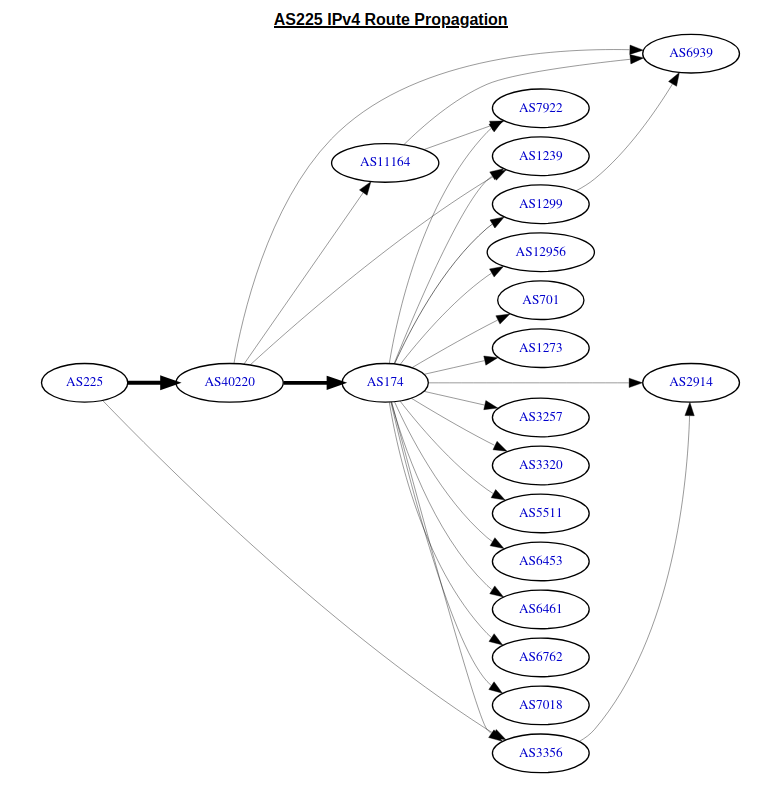
\includegraphics[width=0.5\textwidth]{../routing/as225-graph}
\end{frame}

\begin{frame}{AS40220}
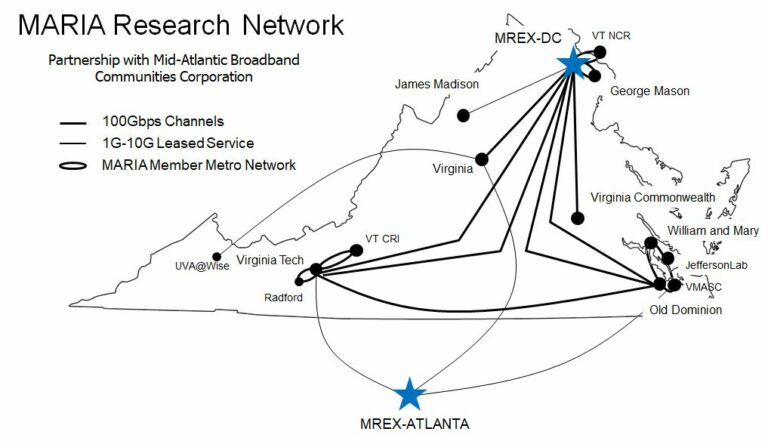
\includegraphics[height=0.8\textheight]{../routing/MARIA-Network-BW-768x441.jpg}
\end{frame}

\begin{frame}{}
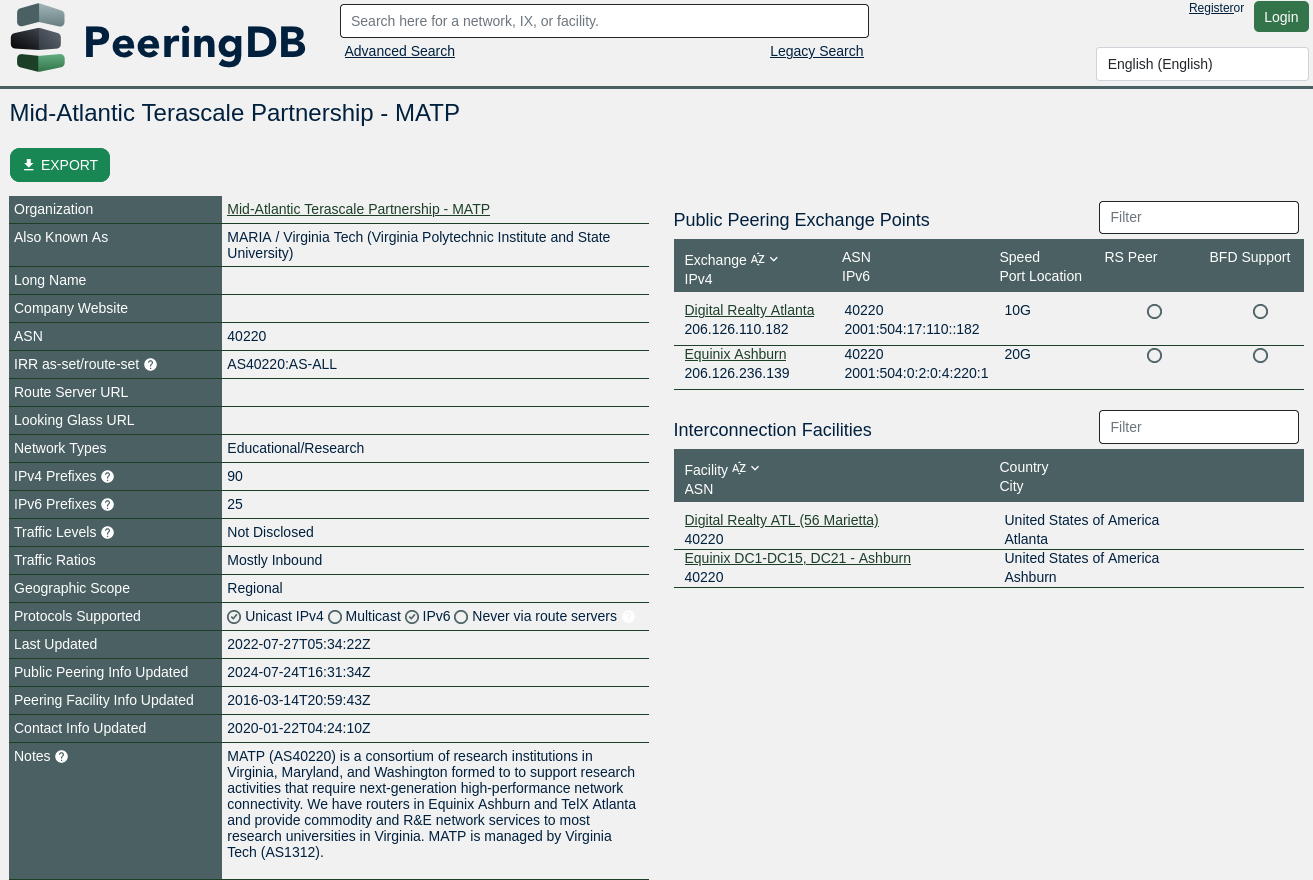
\includegraphics[width=0.95\textwidth]{../routing/as40220-peeringdb}
\end{frame}

\begin{frame}{AS3356}
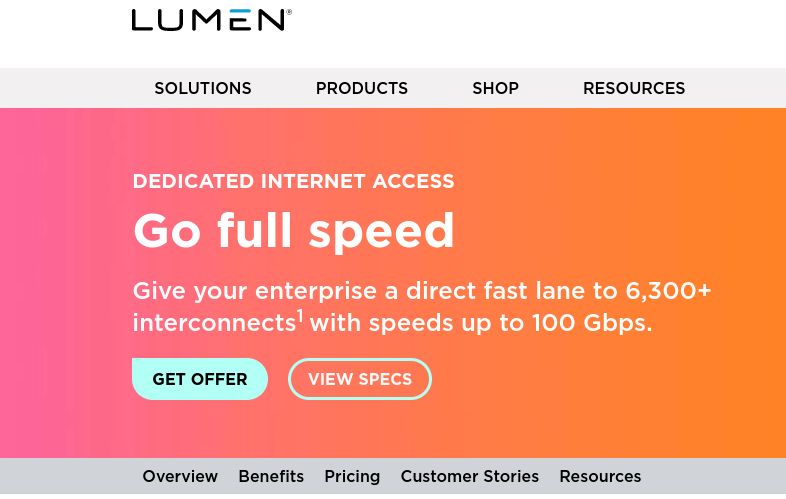
\includegraphics[height=0.8\textheight]{../routing/lumen-webpage.png}
\end{frame}

\begin{frame}{AS3356 is a backup (8x AS prepending)}
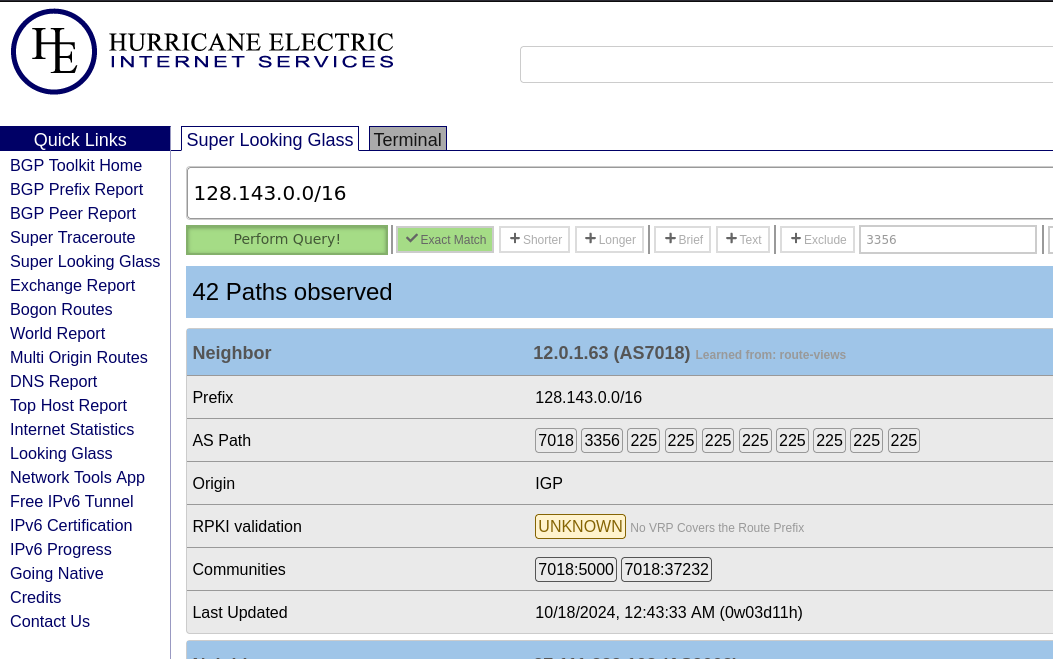
\includegraphics[height=0.8\textheight]{../routing/as3356-he-superlg.png}
\end{frame}


\subsection{internet exchanges, peeringdb}


\begin{frame}{peeringdb}
    \begin{itemize}
    \item \url{https://peeringdb.com} --- commonly used database of ASes and how to peer with them
    \item there is also -- ``whois'' records (from RIRs) for ASes, IP blocks with contact info
    \end{itemize}
\end{frame}

\begin{frame}{internet exchanges and route servers}
    \begin{itemize}
    \item internet exchange
        \begin{itemize}
        \item local network (typically within metro area) for connecting networks
        \item often run at and/or by `carrier-neutral' datacenter
        \item typically high bandwidth (10-100Gbps ports to network)
        \item provides connections when
        \end{itemize}
    \vspace{.5cm}
    \item route servers
        \begin{itemize}
        \item BGP servers run by internet exchange
        \item consolidates routes from participants
        \item goal: only need O($n$) BGP connections, not O($n^2$)
        \end{itemize}
    \end{itemize}
\end{frame}


\subsection{BGP communities}
\begin{frame}{BGP communities}
    \begin{itemize}
    \item routes sent via BGP can have `communities'
    \item extra information tagged on routes sent via BGP
    \vspace{.5cm}
    \item large ISPs have lists of communities their customers/peers can use
    \item \ldots and these affect how those routes are used
    \end{itemize}
\end{frame}

\begin{frame}{aside: Internet2}
    \begin{itemize}
    \item non-profit networking consortium
    \item operations major US University-focused network
    \item basically one of UVa's ISPs
    \end{itemize}
\end{frame}

\begin{frame}[fragile]{selected Internet2 BGP communities}
\begin{tikzpicture}
\node (a) {
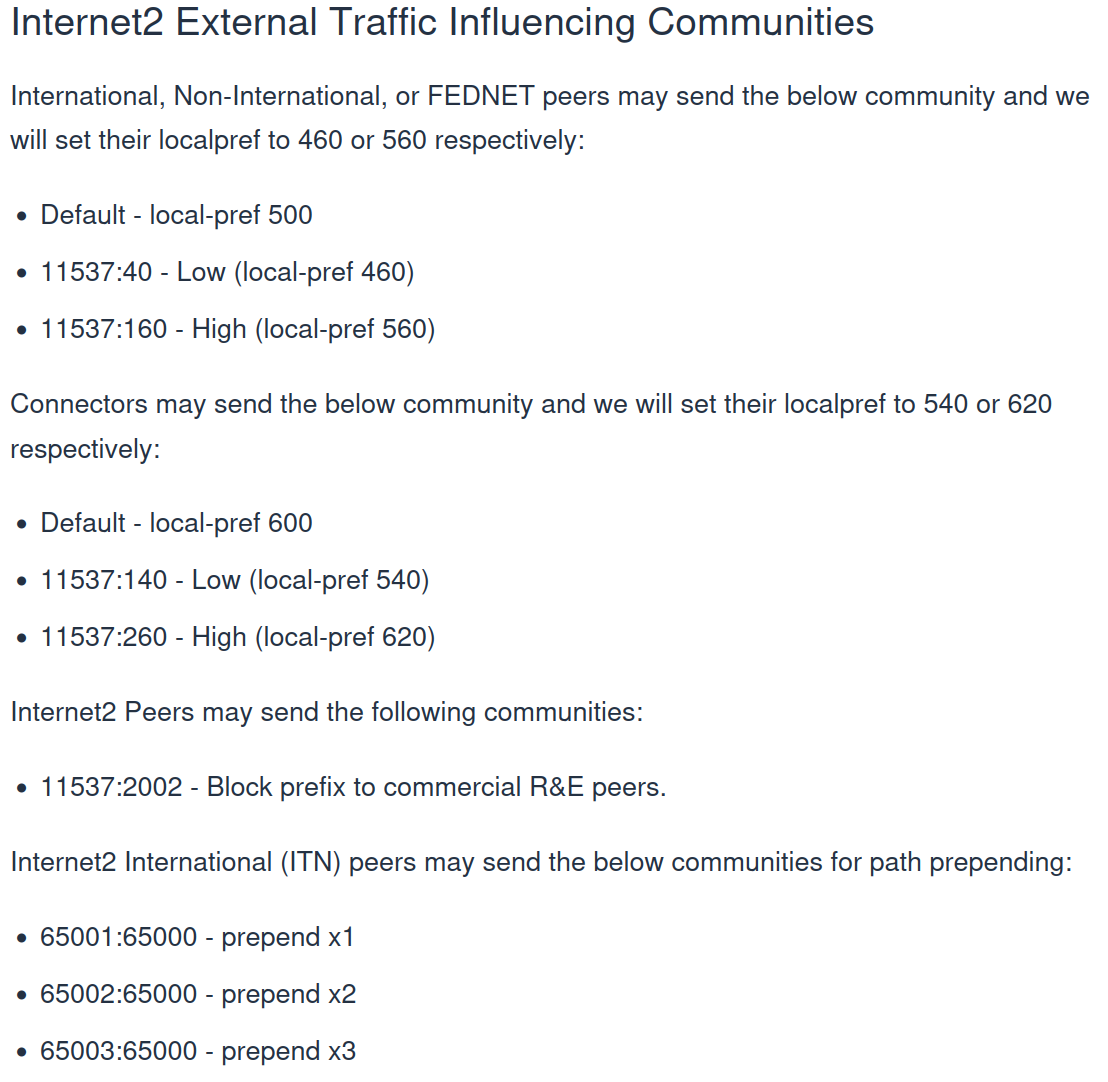
\includegraphics[width=0.49\textwidth]{../routing/i2-bgp-ext-comm}
};
\node[anchor=north west] (b) at (a.north east) {
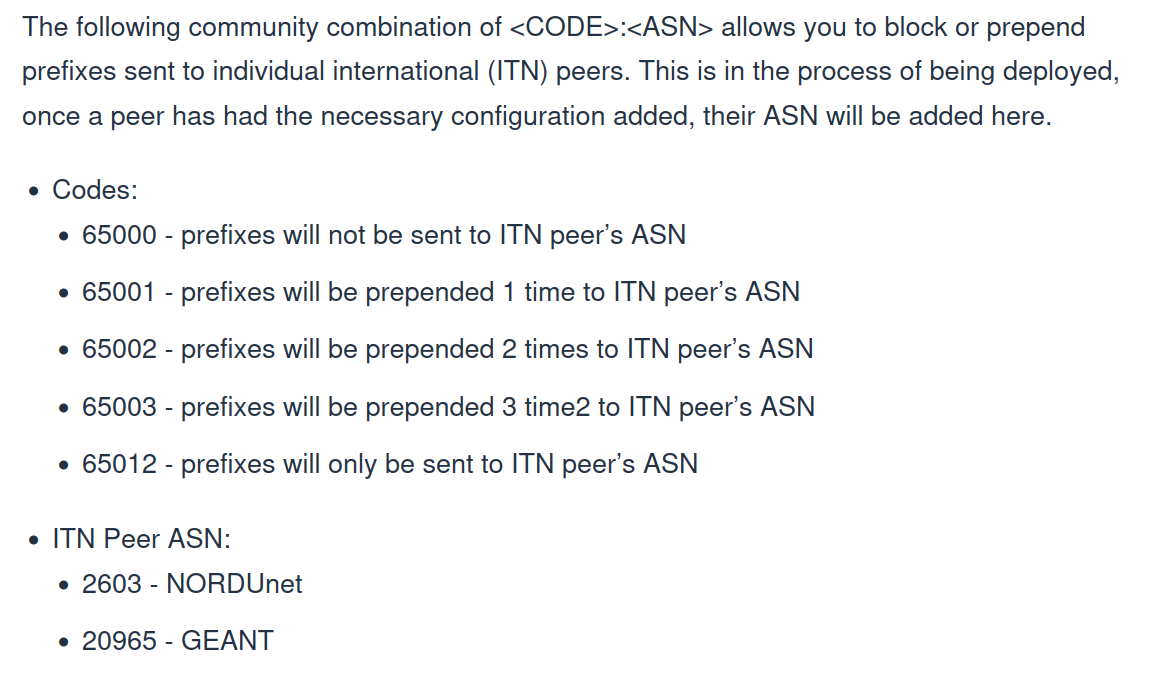
\includegraphics[width=0.39\textwidth]{../routing/i2-bgp-ext-comm2}
};
\node[anchor=north west] (c) at (b.south west) {
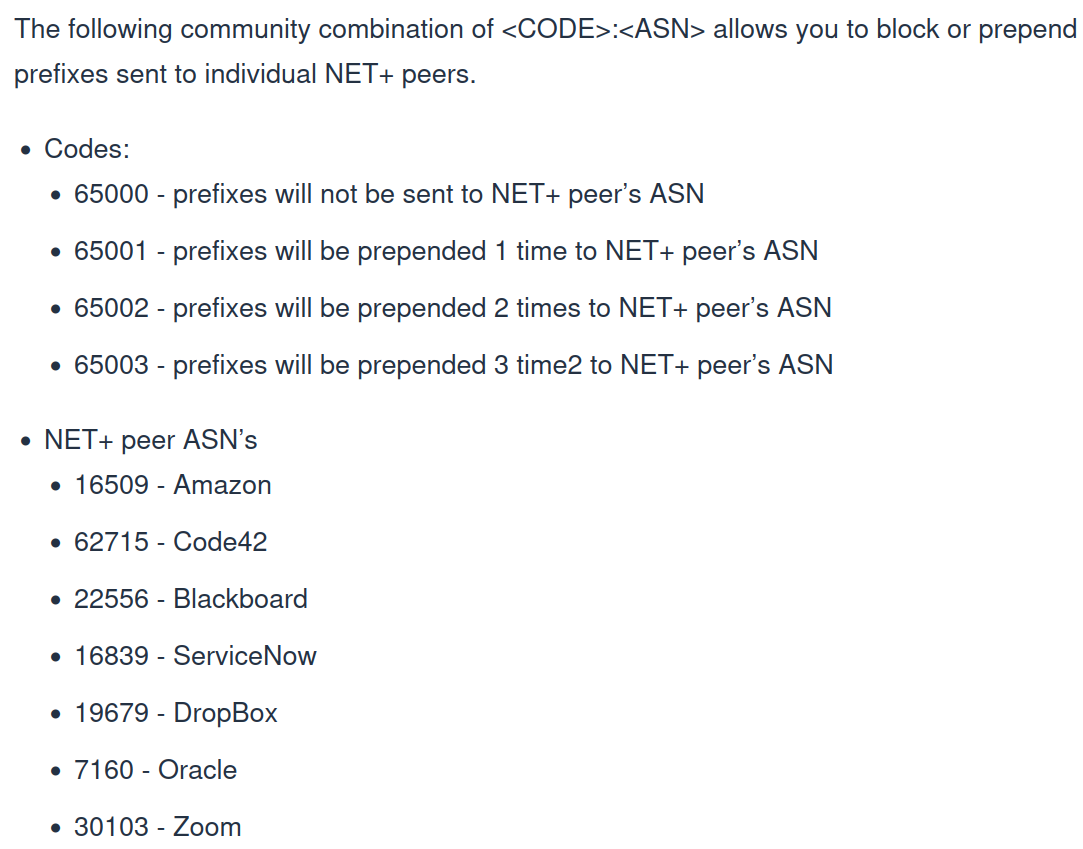
\includegraphics[width=0.39\textwidth]{../routing/i2-bgp-ext-comm3}
};
\end{tikzpicture}
{\fontsize{9}{10}\selectfont\url{https://noc.net.internet2.edu/knowledge/policy-statements/internet2-bgp-communities.html}}
\end{frame}

\begin{frame}{community options from prev slide}
\begin{itemize}
\item setting local-pref:
    \begin{itemize}
    \item you can decide how preferred your route is by Internet2
    \item maybe to make one primary, another secondary?
    \end{itemize}
\item blocking route from being sent to specific place
\item prepending Internet2's AS before forwarding prefix
    \begin{itemize}
    \item hopefully make that route less preferred by others
    \end{itemize}
\item prepending Internet2's AS before forwarding prefix to specific place
    \begin{itemize}
    \item hopefully make that route less preferred by that place
    \end{itemize}
\end{itemize}
\end{frame}

\begin{frame}{other things with communities}
    \begin{itemize}
    \item Internet2 also uses communities to mark\ldots
    \item what location routes were learned from
    \item what type of organization routes were learned from
    \item whether Internet2 is only allowed to use the route non-commerically or not
    \item \ldots
    \end{itemize}
\end{frame}



\subsection{BGP hijacking/fat fingers}

\begin{frame}{AS7007}
{\fontsize{8}{9}\selectfont\url{https://seclists.org/nanog/1997/Apr/444}}

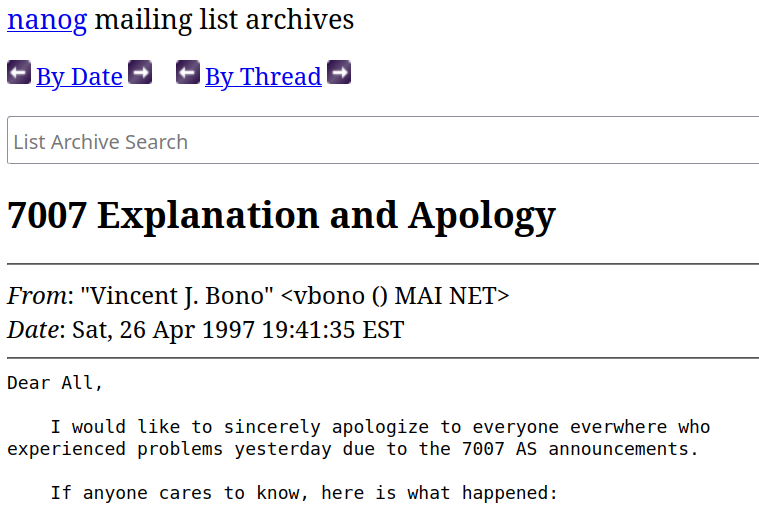
\includegraphics[width=0.4\textwidth]{../routing/as7007-1.png}
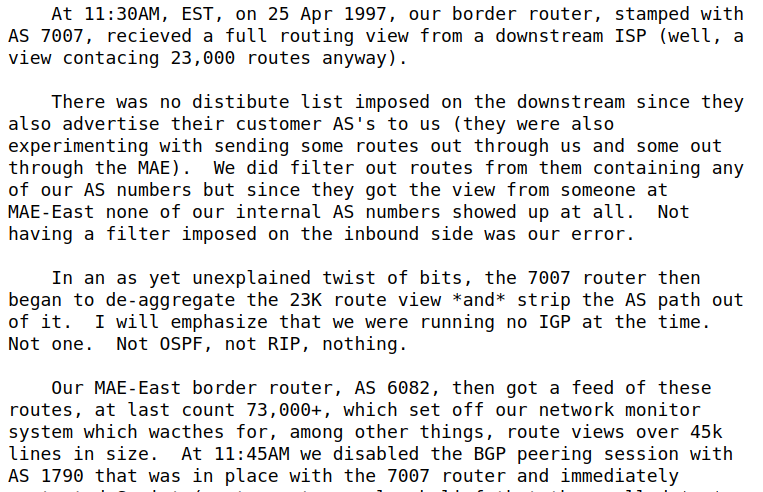
\includegraphics[height=0.4\textwidth]{../routing/as7007-2.png}
\end{frame}

\begin{frame}{2008 Pakistan Youtube}
\begin{itemize}
\item Pakistan Telecom recieved gov't order to block youtube
\item implemented by inserting route for YouTube's IP in internal network
\vspace{.5cm}
\item misconfiguration meant route was advertised on BGP
\item was more specific than YouTube's route, so made YouTube unreachablej
\end{itemize}
\end{frame}

\begin{frame}{timeline from RIPE NCC}
\begin{itemize}
\item {\tiny \url{https://www.ripe.net/about-us/news/youtube-hijacking-a-ripe-ncc-ris-case-study/}}
\item Youtube is announcing 208.65.152.0/22
\item 18:47Z: Pakistan Telecom starts announcing 208.65.153.0/24
\item 20:07Z: Youtube starts announcing 208.65.152.0/24
\item 20:18Z: Youtube starts announcing 208.65.152.0/25 and 208.65.152.128/25
\item 20:51Z: Pakistan Telecom's ISP forwards their announcements with additional copy of Pakistan Telecom's AS number
\item 21:01Z: Pakistan Telecom's ISP withdraws routes initiated by Pakistan Telecom (but not Pakistan Telecom's customers)
\end{itemize}
\end{frame}

\begin{frame}{BGP Hijacking targeted cryptocurrency stuff}
    \begin{itemize}
    \item KLAYswap (Feb 2022), Celer Bridge (Sep 2022)
    \item attackers intentionally redirected traffic to malicious version of services
    \item \ldots and stole money
    \vspace{.5cm}
    \item both probably spoofed the final AS number in AS path
    \item sometimes involved adding attacked IP range to routing registry
    \end{itemize}
\end{frame}

\begin{frame}{nation-states?}

\includegraphics[width=\textwidth]{../routing/china-tele-ars-tech}
\end{frame}


\subsection{validating routes / sBGP}
\begin{frame}{route security}
    \begin{itemize}
    \item historically, no verification routes announced by ``owner'' of IP addresses
    \vspace{.5cm}
    \item probably some ISPs filter
    \item effort to deploy RPKI --- public-key based scheme to verify routes
        \begin{itemize}
        \item checks that routes originated at correct AS
        \item doesn't verify intermediate ASes will forward correctly
        \end{itemize}
    \end{itemize}
\end{frame}

\begin{frame}{}
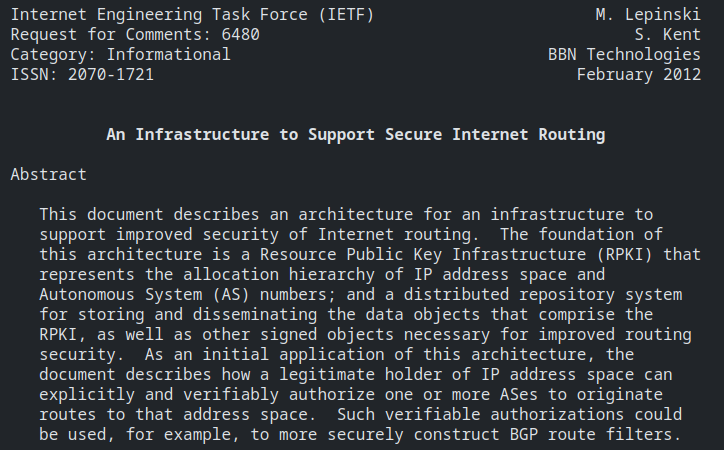
\includegraphics[height=\textheight]{../routing/rpki-rfc}
\end{frame}



\subsection{aside: partial tables}
\begin{frame}{partial tables}
    \begin{itemize}
    \item dealing with full Internet routing table is expensive
    \vspace{.5cm}
    \item common shortcut if you have a couple ISPs:
    \item keep `short' routes (example: short AS path)
    \item use default route for other cases
        \begin{itemize}
        \item to one of your ``primary'' ISPs
        \item maybe using ECMP
        \end{itemize}
    \end{itemize}
\end{frame}


\section{backup slides}
\begin{frame}\frametitle{backup slides}
\end{frame}

\end{document}
